
\chapter{Resultate}\label{results}

Aus diesem Projekt entspringen zwei Resultate. Das erste ist ein bereinigter
Datensatz der gesammelten Texte aus dem Vorprojekt. Das zweite ist die Extraktion
und die Aggregation der Zitate nach Geschlecht und Portal aus den verbleibenden Daten.

\section{Datenbereinigung}

Die Datenbereinigung resultierte in einem 5.5\% reduzierten Datensatz mit insgesamt 351'021 Artikeln ohne Duplikate.
Die Abbildung \ref{datenbereinigung} zeigt den Datenstand vor und nach der Entfernung von gleichen oder sehr ähnlichen Texten.
Es war beruhigend festzustellen, dass die Datenbank insgesamt nur wenige Duplikate enthielt.

So fanden wir bei Blick 2'430, bei SRF 2'956, bei Watson 14'895 und bei 20 Minuten 351 doppelte Artikel.

\begin{figure}[H]
	\begin{center}
        \centering
		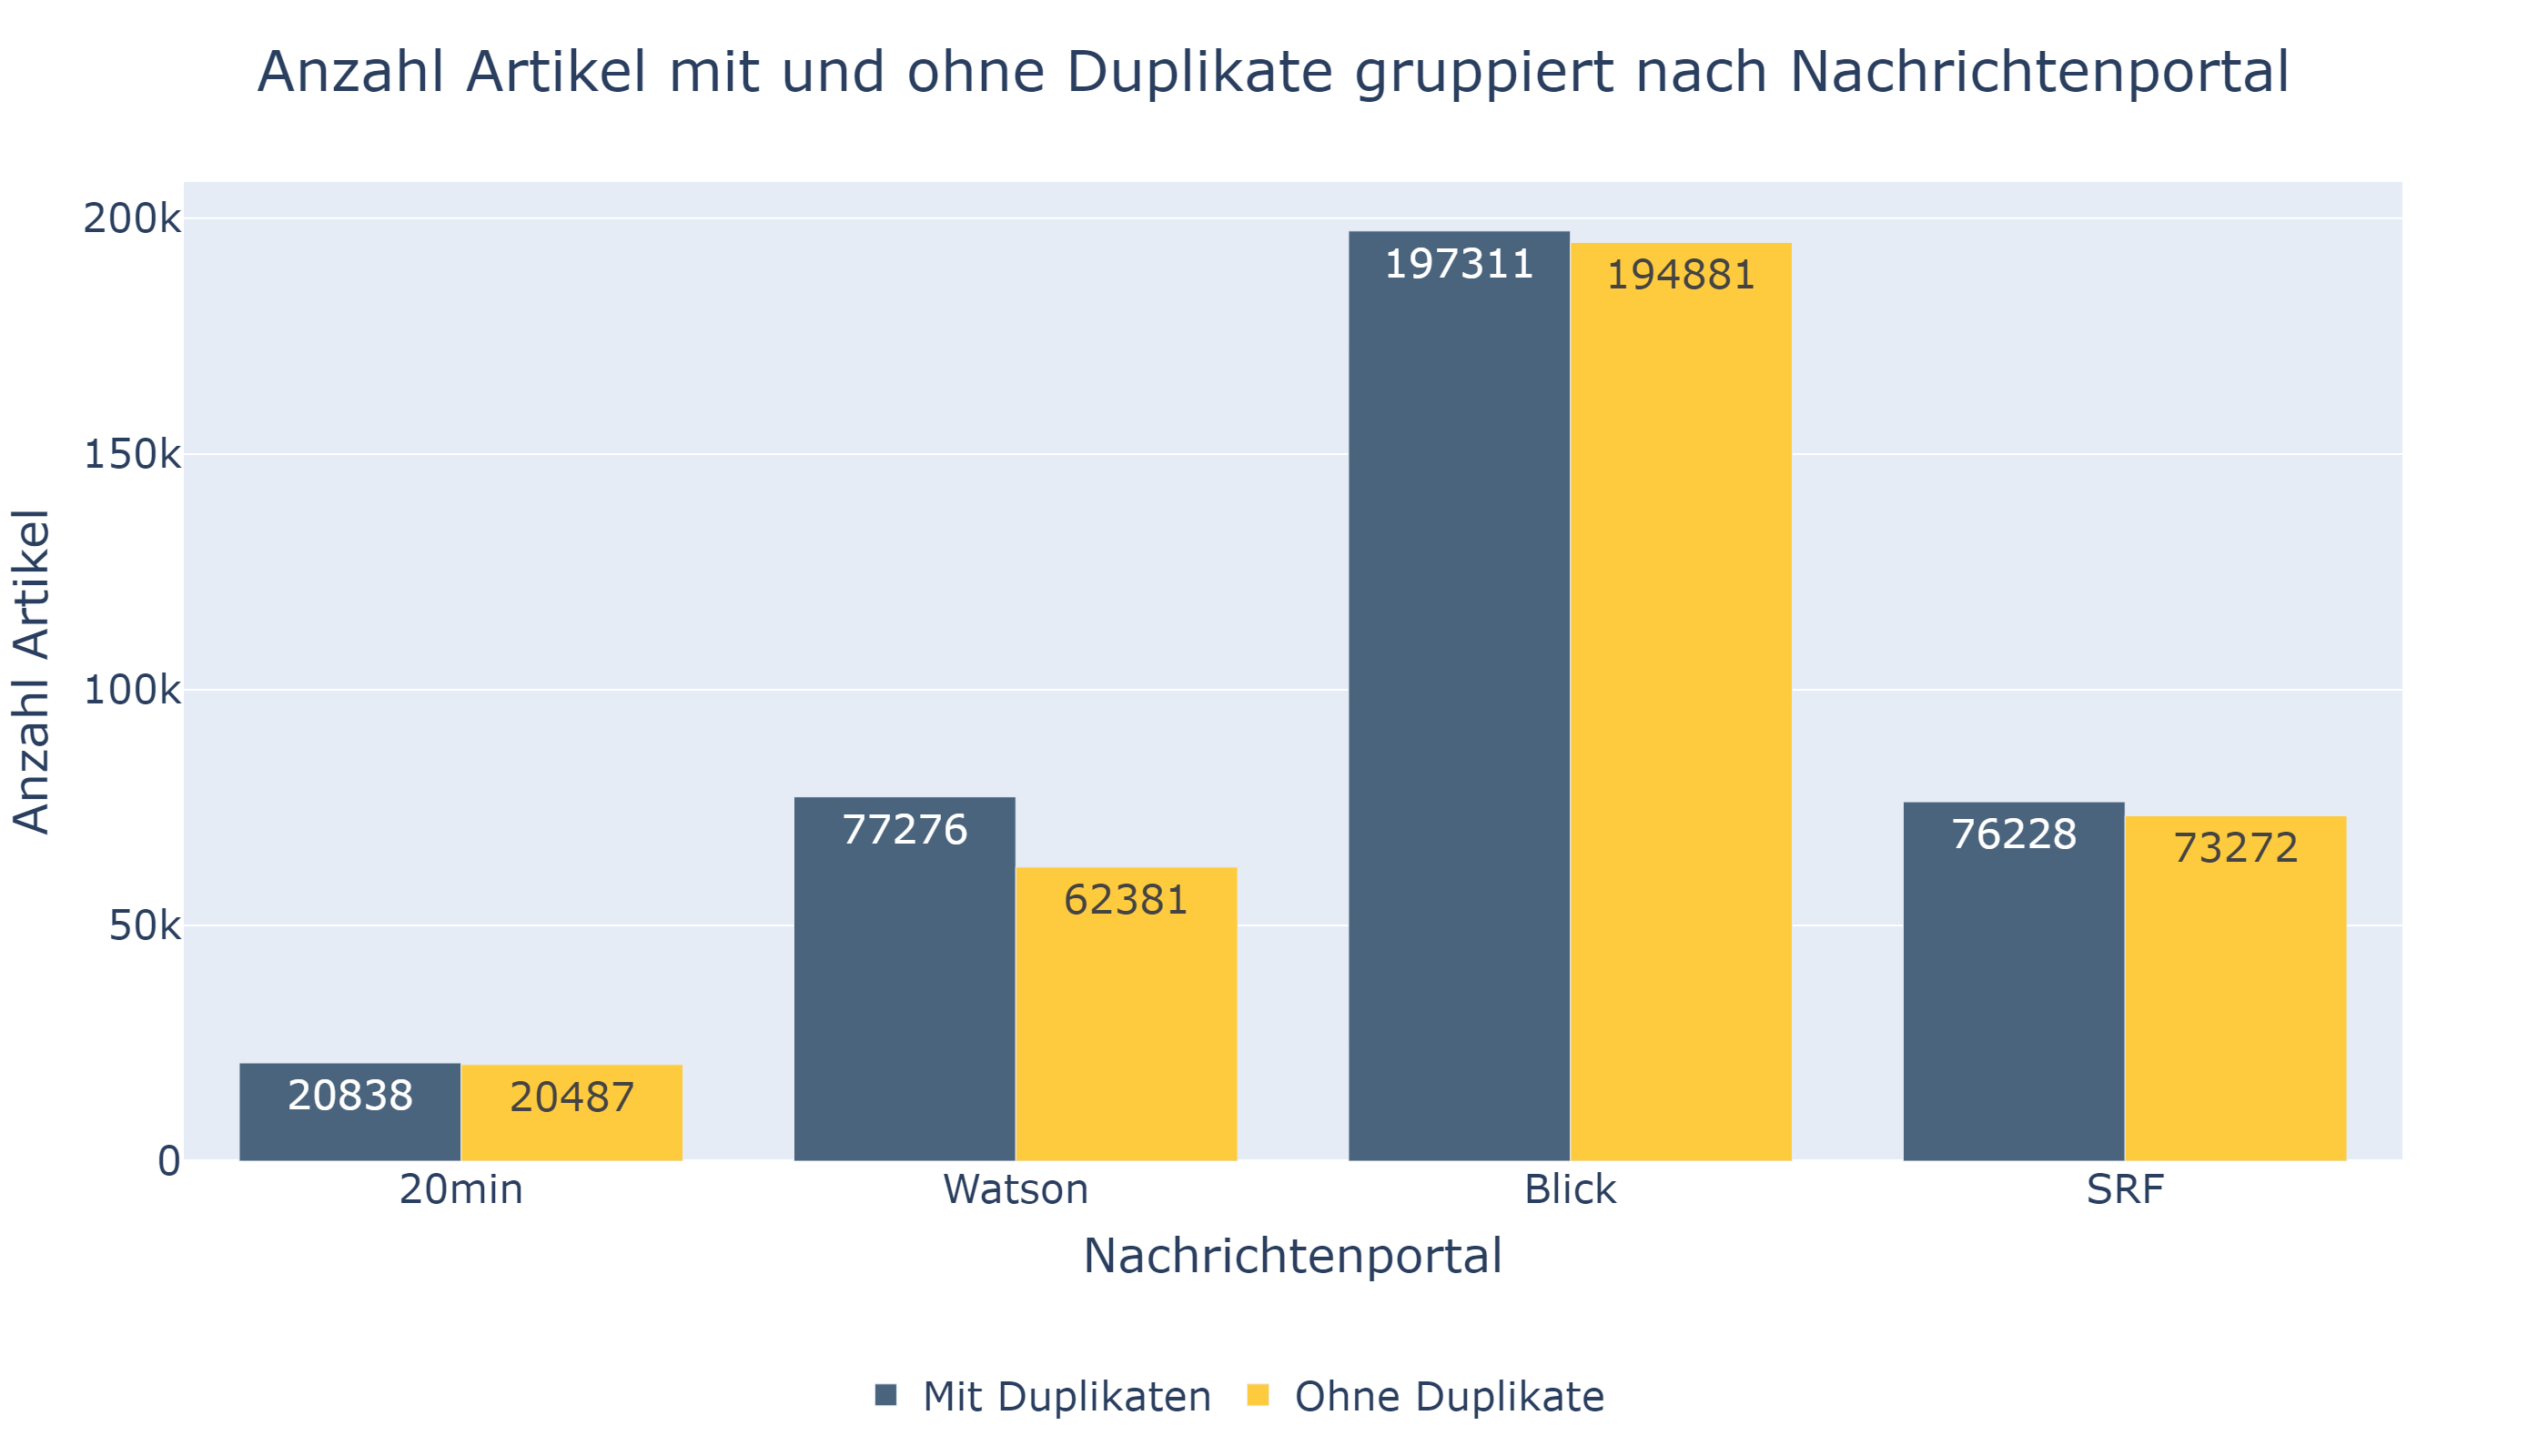
\includegraphics[width=1\linewidth]{./images/datenbereinigung.png}
		\caption{Anzahl Artikel vor und nach der Datenbereinigung}
		\label{datenbereinigung}
	\end{center}
\end{figure}

\section{Extraktion und Aggregation der Zitate}

Die folgenden zwei Abschnitte beschreiben die Verteilung der gefundenen Zitate pro
Nachrichtenportal und in einem weiteren Schritt zusätzlich pro Geschlecht. Der letztere Teil
beantwortet eigentliche Forschungsfrage zum \gl{gendergap}.

\subsection{Verteilung der Zitate pro Nachrichtenportal}

Das Ergebnis der in Kapitel \ref{citation-extraction} beschriebenen Extraktion der Zitate
resultierte in einer neuen MongoDB \gl{collection} \enquote{analyzed\_articles}. Diese enthält
für jeden Artikel der \gl{collection} \enquote{unique\_articles} die wichtigsten Artikelinformationen
plus die gefundenen Zitate. Insgesamt fanden wir 133'443 Zitate über alle
Nachrichtenportale. Die Grafik \ref{count-citations-per-portal} zeigt die Verteilung über die
Portale.

\begin{figure}[H]
	\begin{center}
        \centering
		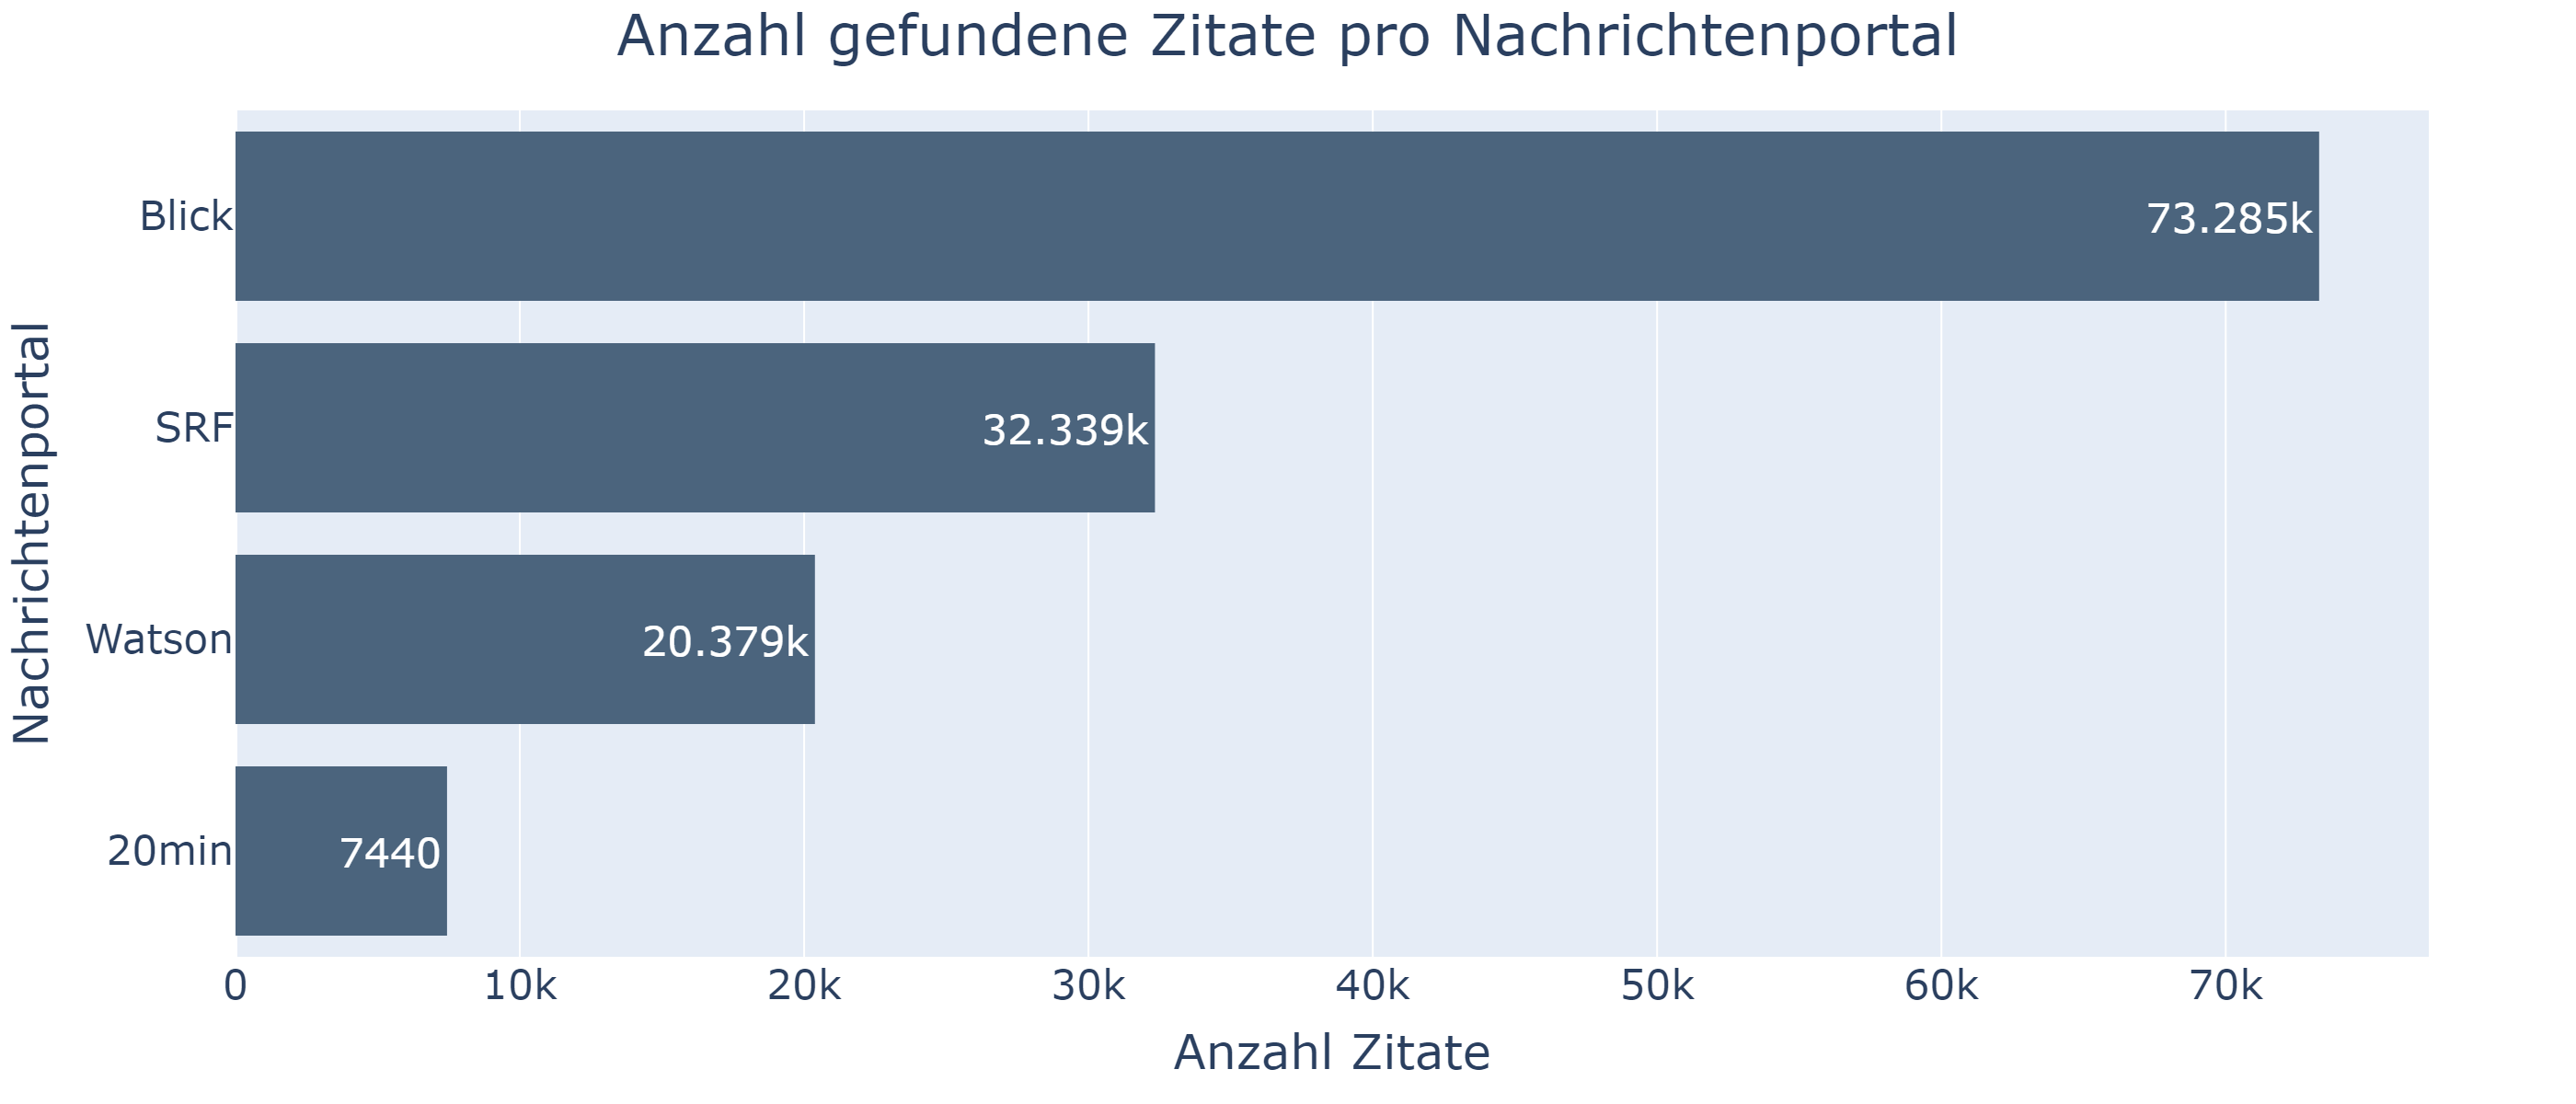
\includegraphics[width=1\linewidth]{./images/plot_anzahl_zitate_pro_portal.PNG}
		\caption{Anzahl gefundene Zitate}
		\label{count-citations-per-portal}
	\end{center}
\end{figure}

Der Algorithmus fand am meisten Zitate von Blick, gefolgt von SRF und Watson und am wenigsten
von 20min. Diese Verteilung ist nicht überraschend, wenn man die Verteilung der Anzahl Artikel bedenkt (vgl. Abbildung \ref{datenbereinigung}).

Eine spannende Erkenntnis ist im Diagramm in Abbildung \ref{citations-per-article} zu sehen,
das die Anzahl gefundener Zitate pro Portal pro Artikel darstellt. Mit einem Quotienten von
0.44 scheint SRF deutlich häufiger Zitate in seinen Artikeln zu verwenden als die anderen. Blick und 20min weisen
mit 0.38 resp. 0.36 einen ähnlichen Wert auf. Watson weist mit 0.33 Zitate den kleinsten Wert auf.

\begin{figure}[H]
	\begin{center}
        \centering
		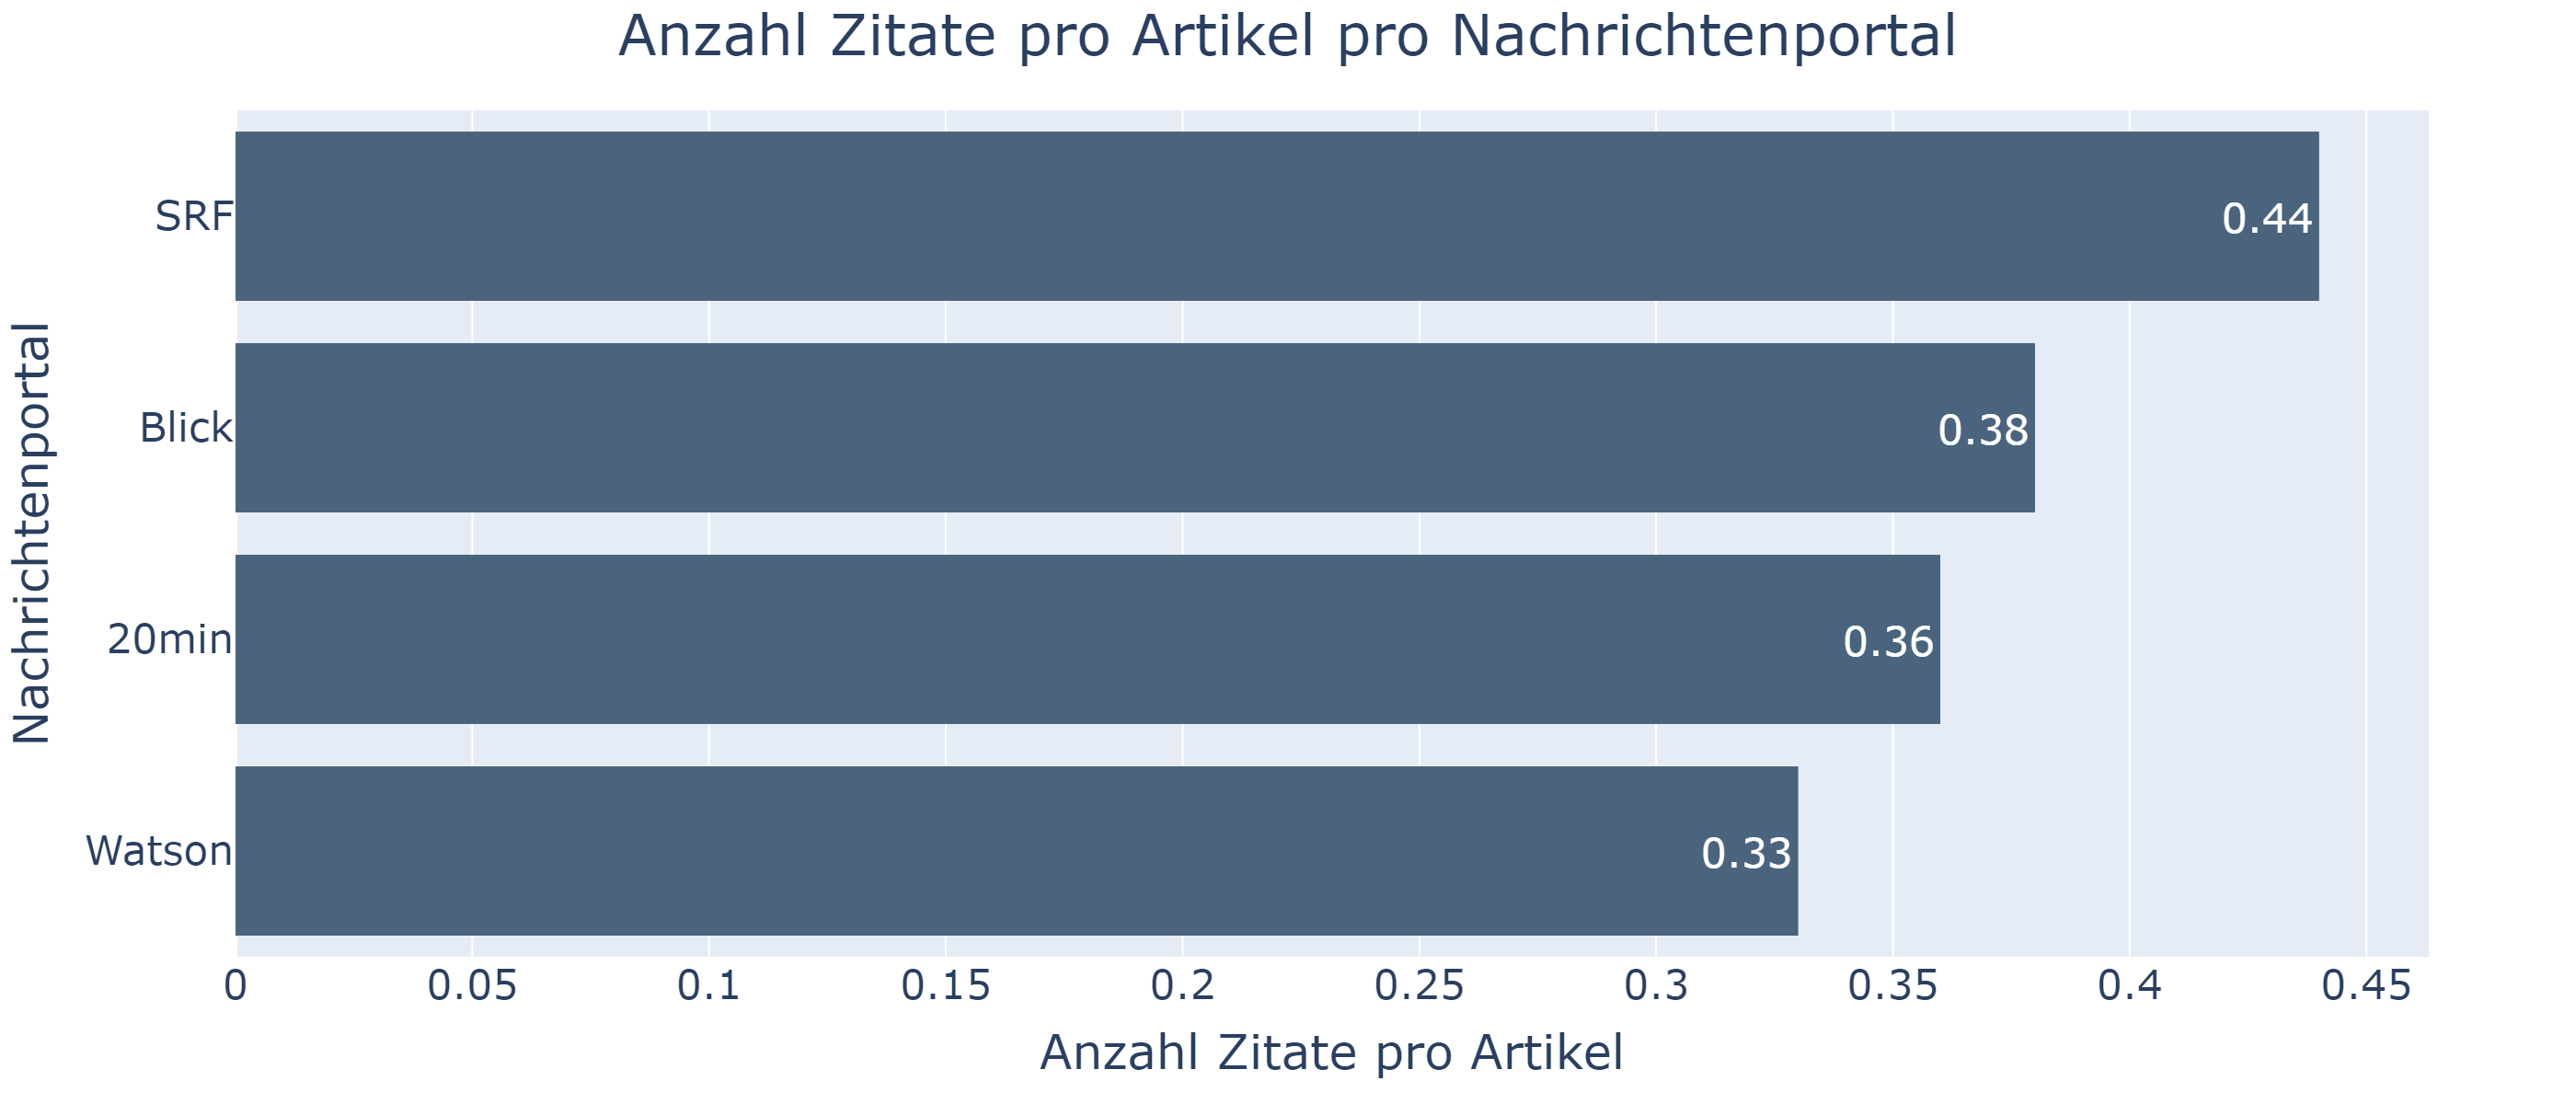
\includegraphics[width=1\linewidth]{./images/plot_zitate_pro_artikel.PNG}
		\caption{Anzahl gefundene Zitate pro Artikel pro Nachrichtenportal}
		\label{citations-per-article}
	\end{center}
\end{figure}



\subsection{Verteilung der Zitate pro Nachrichtenportal und pro Geschlecht}

Bevor wir in die Auswertung zum \gl{gendergap} in den Nachrichtenportalen eintauchen, möchten
wir nochmals betonen, dass die Zahlen ausschliesslich die auf unserem Datensatz gemessenen Resultate darstellen
und diese eine potenziell grosse Ungenauigkeit aufweisen (vgl. Kapitel \ref{quality-assurance}).

Gruppiert nach dem identifizierten Geschlecht ergibt sich eine Verteilung, die auf eine starke
Übervertretung von Zitaten von Männern hindeutet, wie die Abbildung \ref{sum-citations-stacked} zeigt.
So scheinen alle Nachrichtenportale eine ähnliche Verteilung aufzuweisen, in der gut zwei Drittel
der Zitate von Männern stammen und nur ein Fünftel oder ein Viertel von Frauen. Der Rest ist entsprechend
\enquote{unbekannt} zugeordnet. Diese Zuordnung bedeutet, dass der Algorithmus das Geschlecht der zitierten Person nicht ausfindig machen konnte.
Das arithmetische Mittel über die vier Portale liegt bei den Männern bei 65.6\% und bei den Frauen bei 21.2\%. Hinzu kommen 13.2\% der Kategorie \enquote{unbekannt}.
Diese Werte sind in der Abbildung \ref{sum-citations-stacked} zwischen den Portalen mit dem Label \enquote{Mittelwert} aufgelistet.
Aufgrund der limitierten Qualität (beschrieben im Kapitel \ref{quality-assurance})
können die kleinen Unterschiede nicht zum exakten Vergleich oder Ranking zwischen den Portalen verwendet werden.

\begin{figure}[H]
	\begin{center}
        \centering
		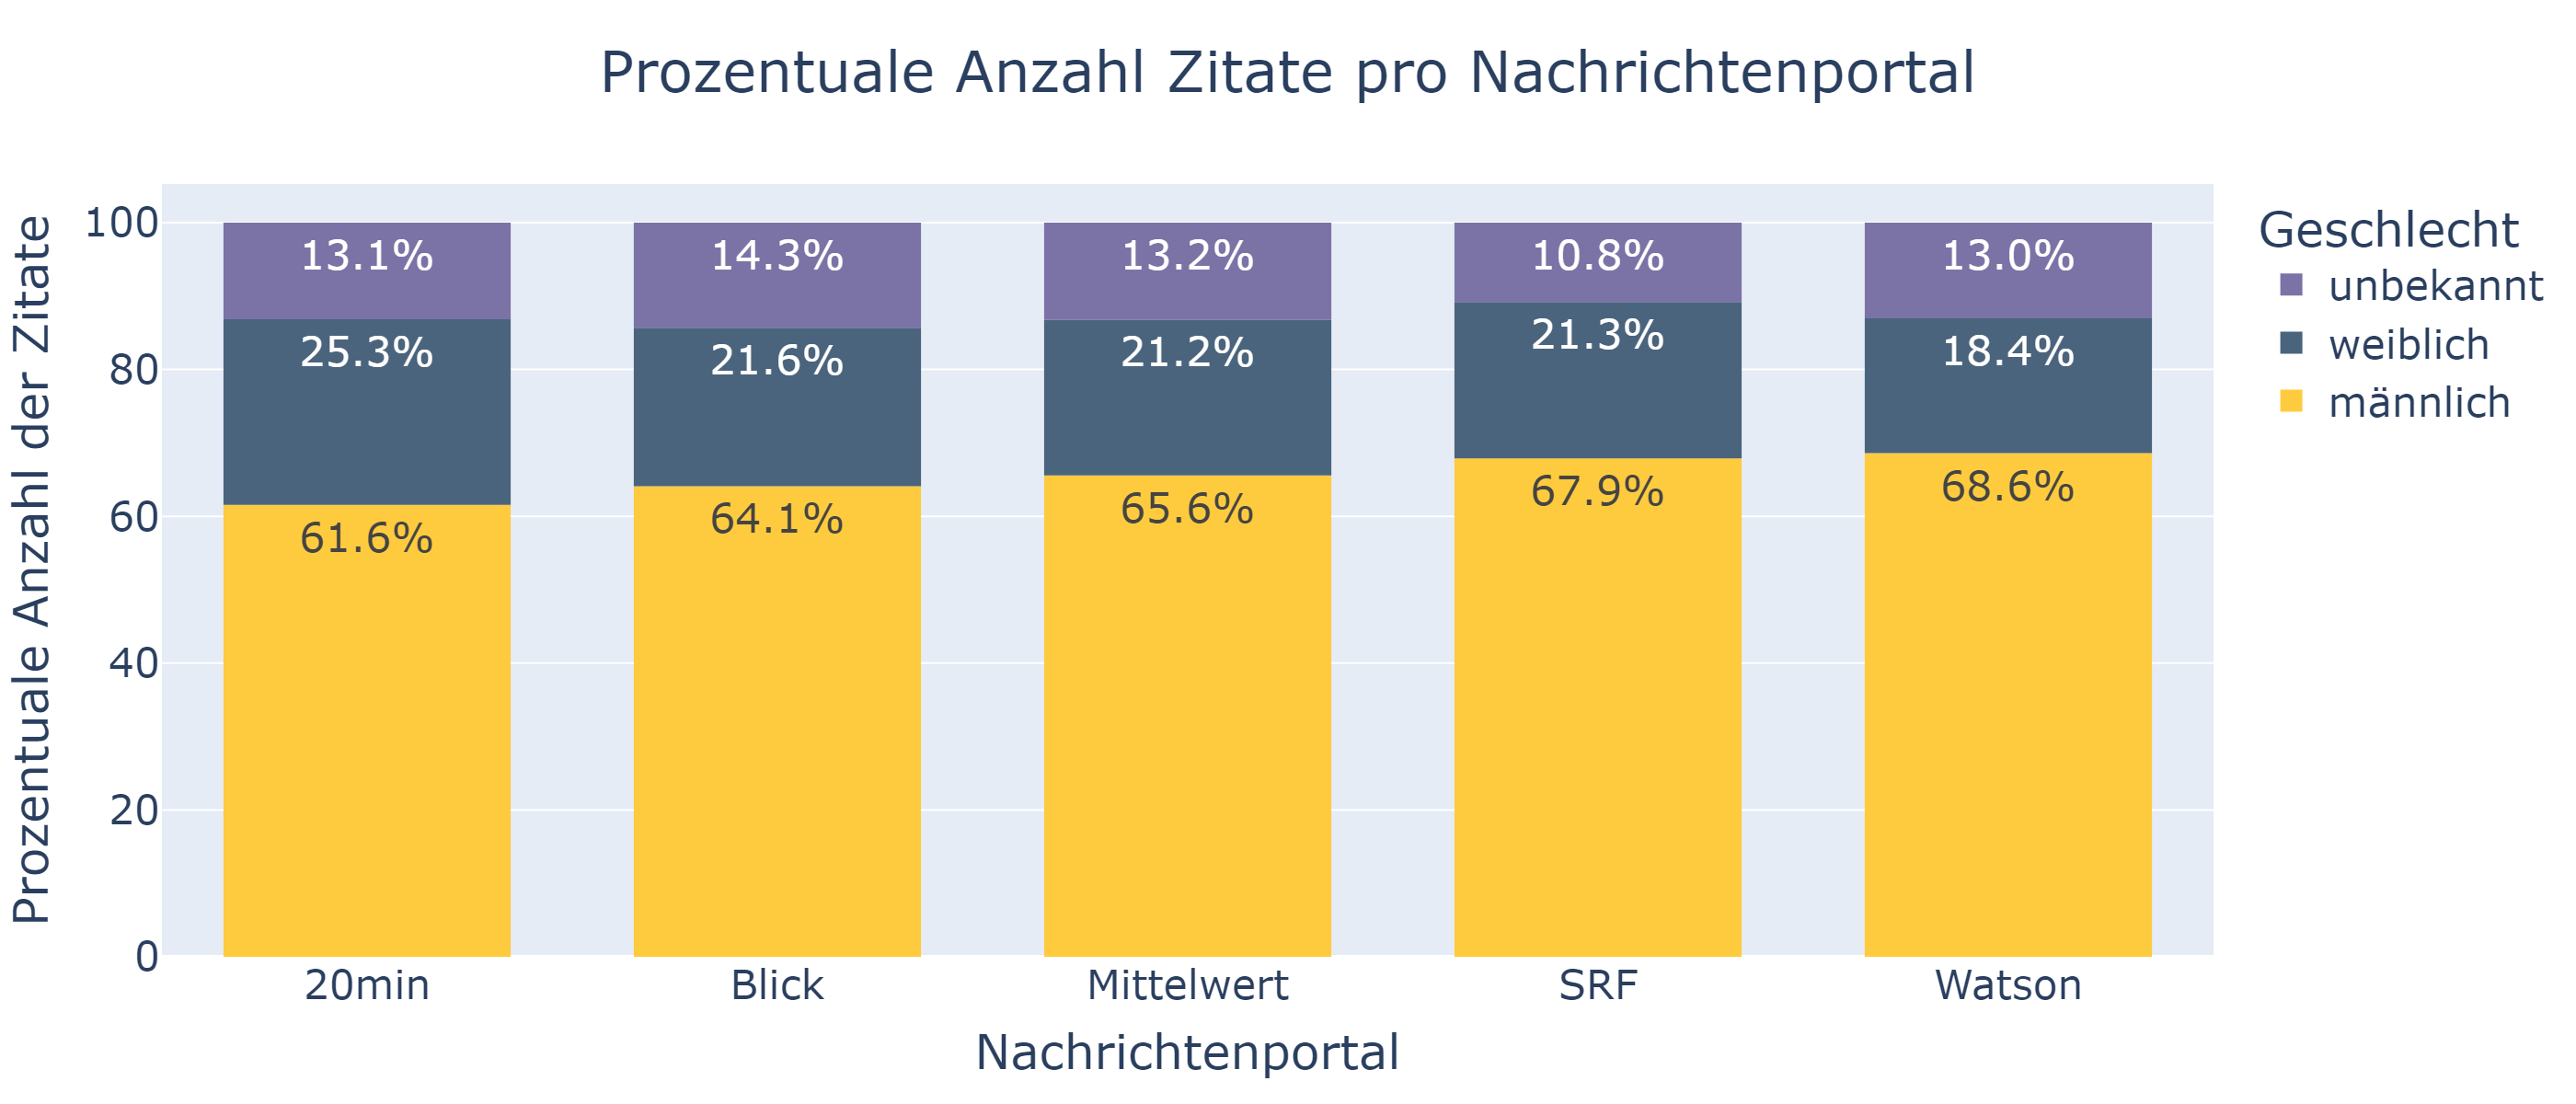
\includegraphics[width=1.1\linewidth]{./images/plot_zitate_pro_portal_geschlecht_stacked_prozentual.PNG}
		\caption{Prozentuale Anzahl Zitate pro Nachrichtenportal}
		\label{sum-citations-stacked}
	\end{center}
\end{figure}

Aufgrund dieser Resultate lässt sich nun endlich der \gl{gendergap} anhand der definierten Formel \ref{ggt-formula}
bestimmen. Dieser ist pro Portal in der Abbildung \ref{gender-gap-per-portal} dargestellt.

Sie zeigt, dass der Algorithmus bei Watson mit 57.7\% den grössten \gl{gendergap} messen konnte. SRF und Blick folgen mit 52.24\%
und 49.59\% respektive. Den kleinsten Gap fand er bei den Artikeln von 20min mit 41.77\%. Das arithmetische
Mittel über die Portale lag bei dieser Kennzahl bei 50.34\%, gekennzeichnet als \enquote{Mittelwert} in der Grafik.

Unter Berücksichtigung der Limitationen (vgl. Abschnitt \ref{limitations}) bedeutet diese Zahl, 
dass Frauen in unserem Datensatz im Schnitt 50.34\% weniger häufig zitiert werden als Männer.

\begin{figure}[H]
	\begin{center}
        \centering
		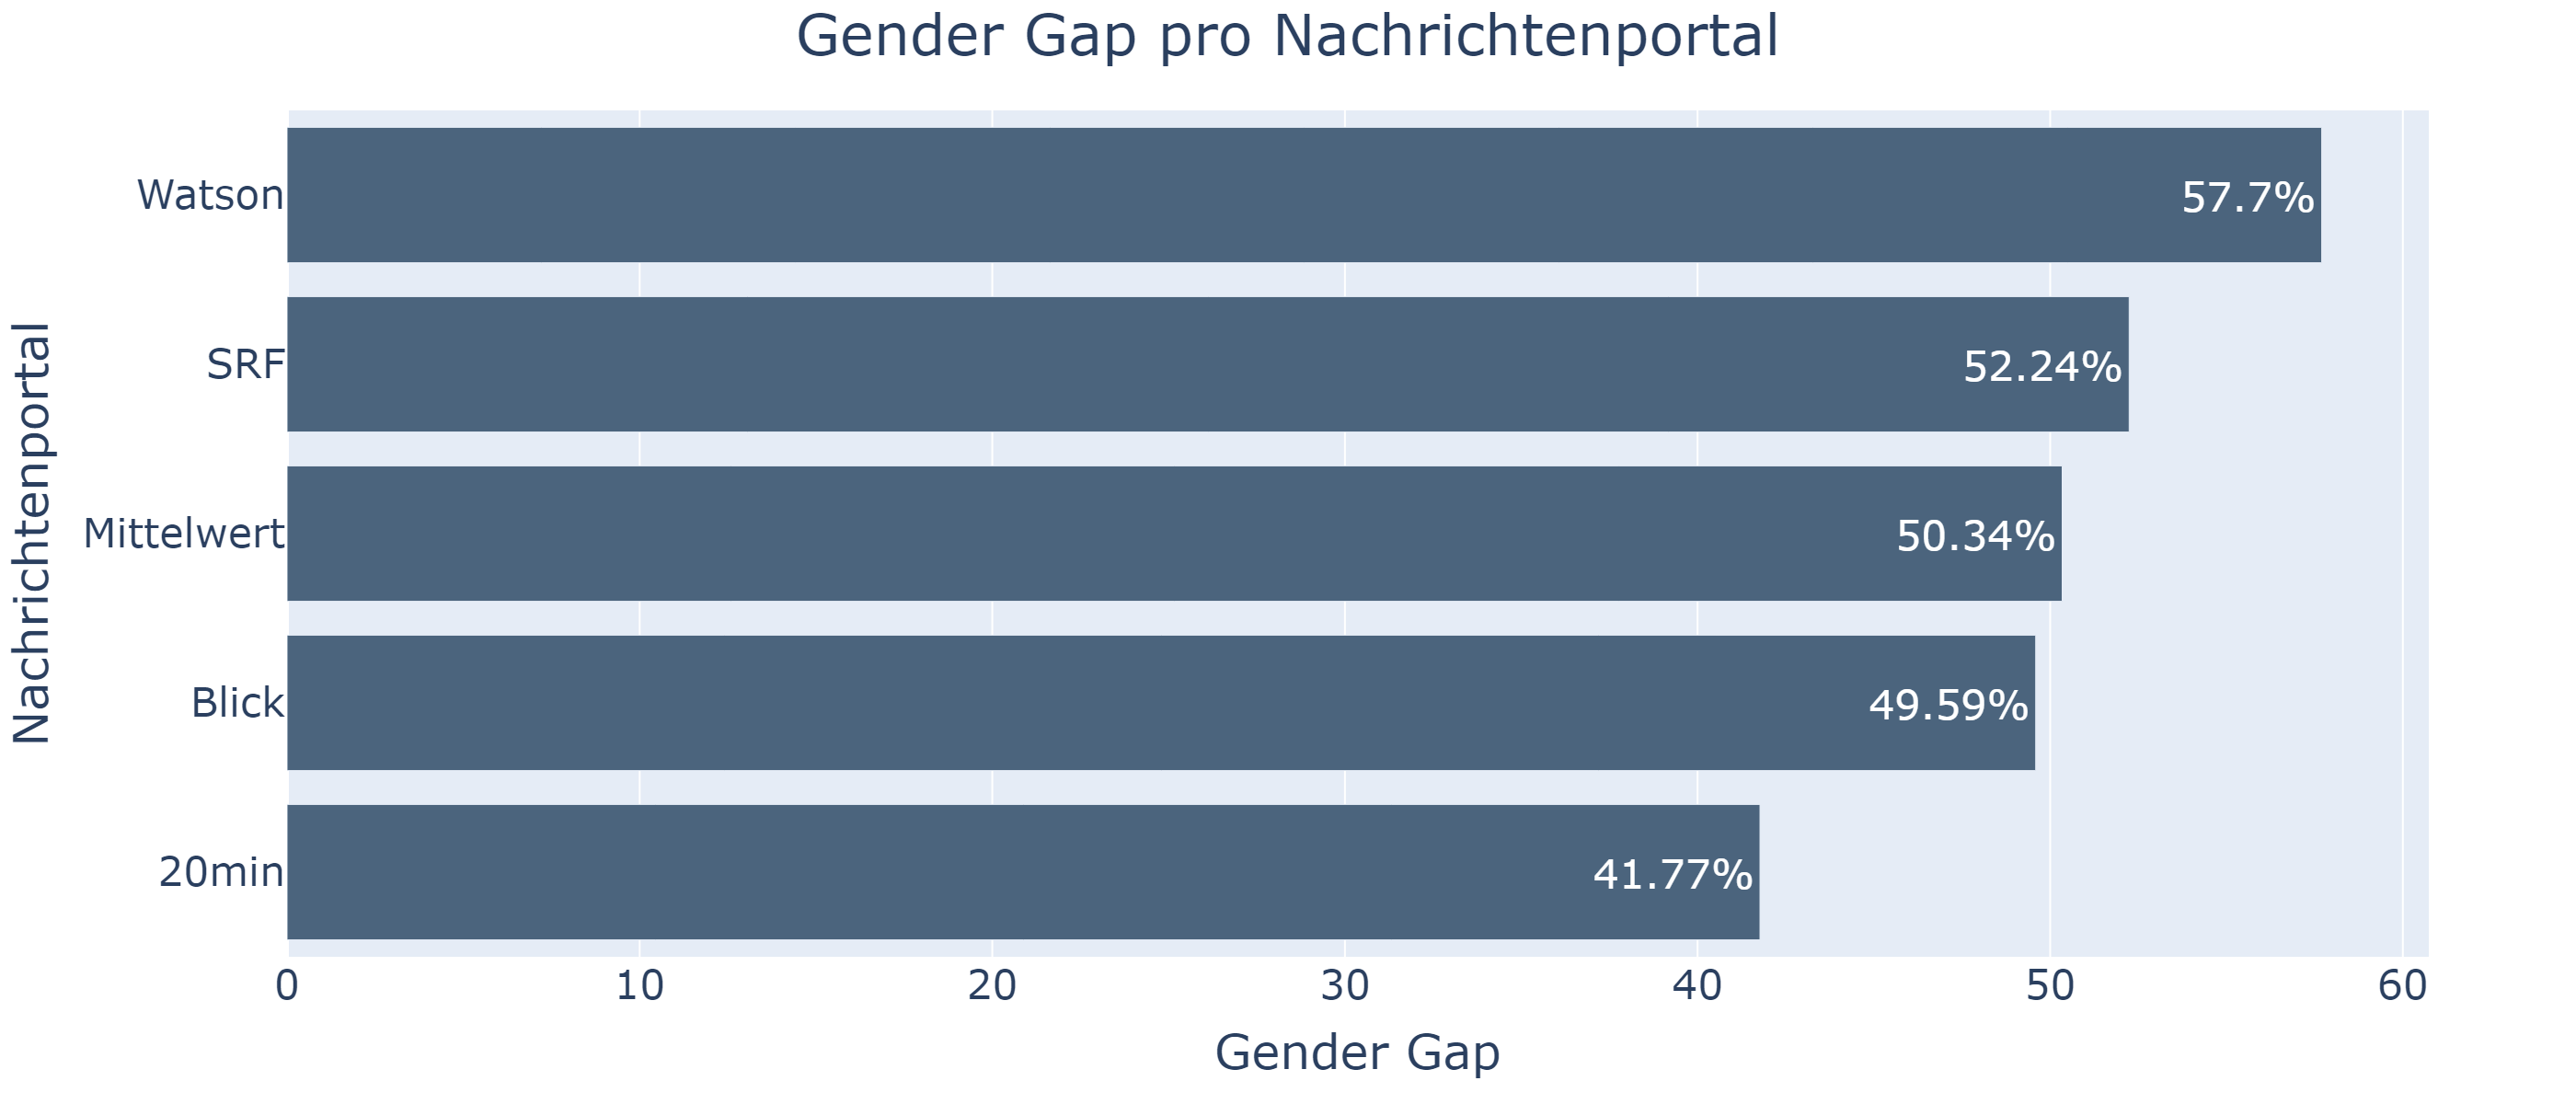
\includegraphics[width=1\linewidth]{./images/plot_gender_gap_pro_portal.PNG}
		\caption{Gender Gap pro Nachrichtenportal}
		\label{gender-gap-per-portal}
	\end{center}
\end{figure}

\section{Qualitätssicherung}\label{quality-assurance}

Die grossen Datenmengen in diesem Projekt verlangten einen methodischen Ansatz zum Validieren der Qualität,
da eine Überprüfung aller Resultate aufgrund der grossen Anzahl und der Zeiteinschränkung nicht machbar war.
Aufgrund des zeitlichen Rahmens war eine systematische Bewertung der Qualität der Ergebnisse
nur bei der Extraktion der Zitate machbar.
Um ein ganzheitlicheres Bild über die Qualität der Auswertung erhalten zu können,
müssten die anderen Teile auch systematisch getestet und bewertet werden.

Die Qualität der Funktionen zum Erkennen der Zitate und Bestimmen des Geschlechts wurden ebenfalls mithilfe von
Gradings sichergestellt. Diese waren besonders während dem Entwickeln relevant und wurden deshalb aus praktischen Gründen
nicht weiter verfeinert. Die Algorithmen funktionieren mit zufriedenstellender Qualität, gemessen an Stichproben,
die wir von Hand durchgeführt haben.

Weil die Extraktion der Zitate im Gegensatz dazu keiner eindeutigen Logik folgen kann, war es für die Entwicklung dieses Algorithmus
wichtig, die Qualität und die Verbesserung des Algorithmus zu messen. Dies ermöglicht es uns ausserdem die Qualität
der Resultate abzuschätzen. 
Ein eigens dafür entwickelter Bewertungsalgorithmus soll einen möglichst guten Überblick über die Anzahl
der gefundenen Zitate und deren Qualität geben.

Dazu haben wir in manueller Arbeit pro Nachrichtenportal fünf Artikel ausgewertet und als JSON abgelegt. Insgesamt ergeben
sich daraus 20 Test-Artikel. Der Bewertungsalgorithmus ruft die Funktionalität zum Extrahieren der Zitate mit dem rohen
Text der Artikel auf und vergleicht das Resultat im Anschluss mit den manuell erstellten Lösungen. Als wichtigste Metrik
dient dabei der \enquote{Recall} (Abbildung \ref{recall-formula}).

\subsection{Recall}

Diese Metrik wird häufig auch im \gl{ml} verwendet, um die Genauigkeit des trainierten
Modells zu messen. Der Recall sagt in unserem Fall aus, wie viele der relevanten Zitate der Algorithmus finden konnte.
Der Recall ist die Prozentzahl der totalen Anzahl Zitate, die er hätte finden können.

\begin{figure}[H]
    \begin{equation}
        Recall = \frac{Anzahl \, gefundene \, Zitate}{Totale \, Anzahl \, Zitate}
    \end{equation}
    \caption{Formel Recall}
    \label{recall-formula}
\end{figure}

Als gefundene Zitate zählt der Bewertungsalgorithmus all diejenigen Zitate, die eine Qualität von
mindestens 60\% aufweisen. Mehr dazu in Kapitel \ref{quality-grade}
Die nachfolgende Abbildung \ref{piechart-recall} visualisiert den Recall von 61.2\% über
alle Nachrichtenportale.
Dieser Wert sagt aus, dass das Programm von allen vorhandenen Zitaten in den Lösungen
61.2\% gefunden hat.

\begin{figure}[H]
	\begin{center}
        \centering
		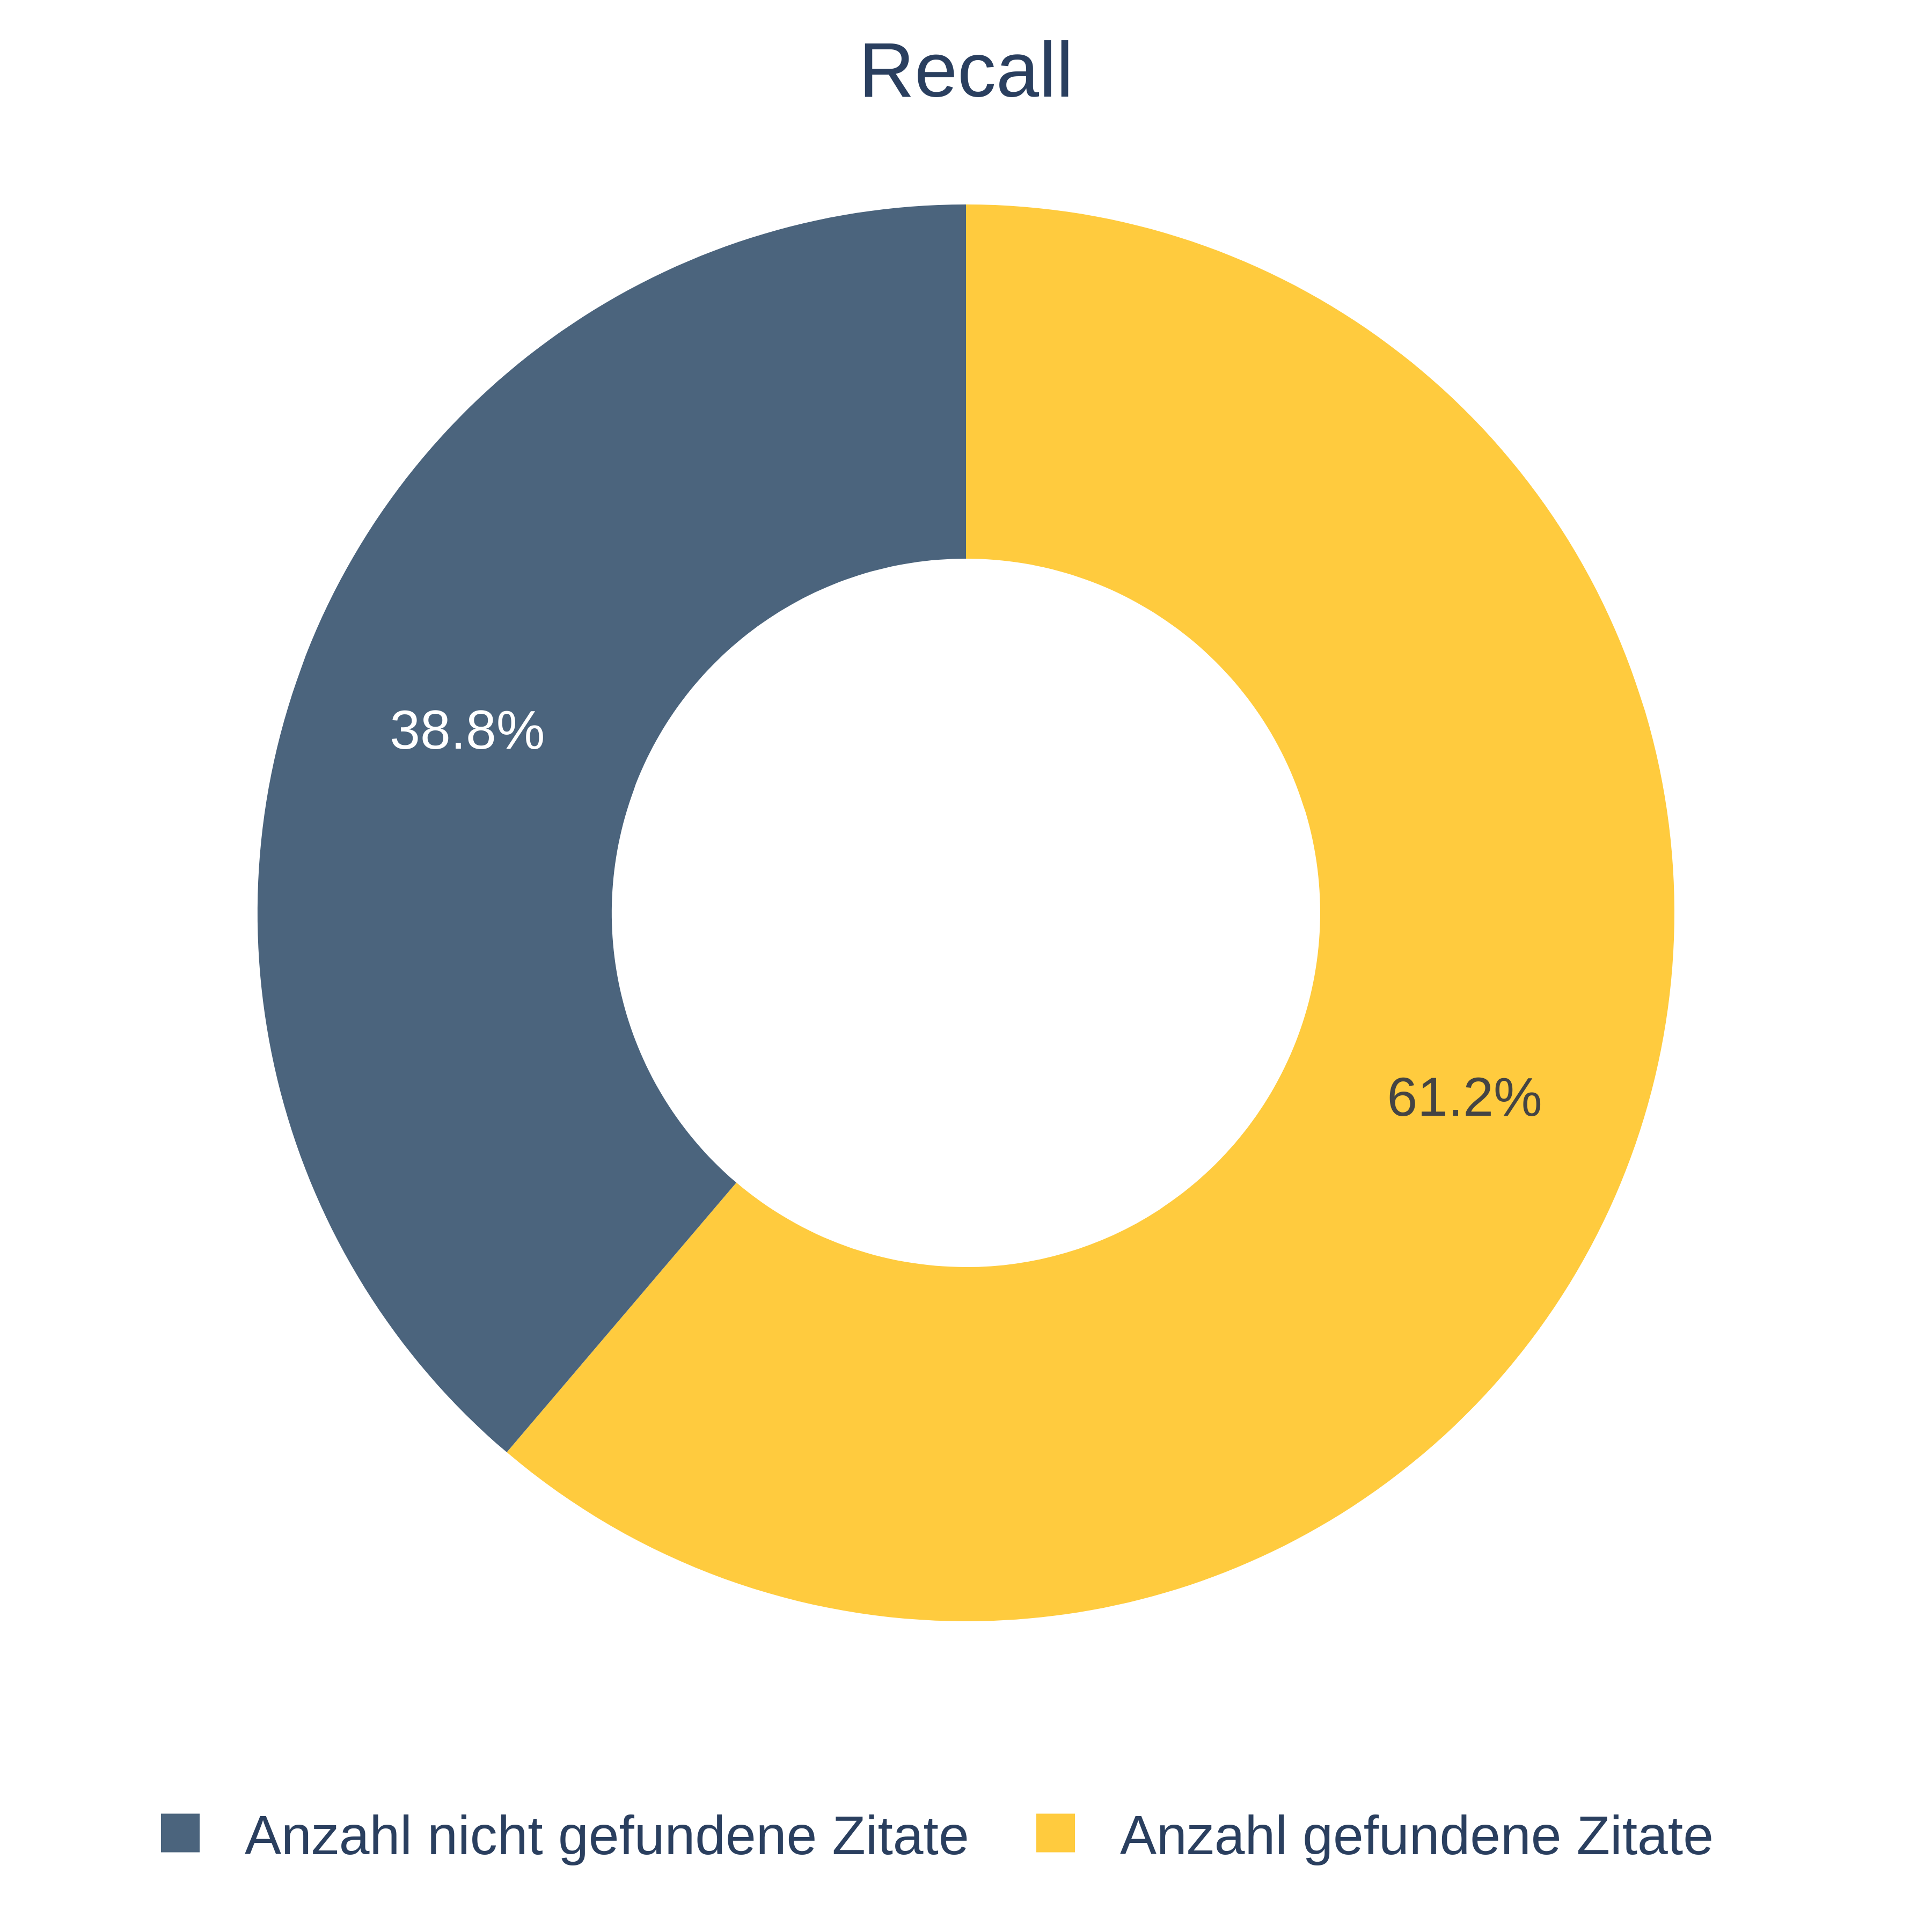
\includegraphics[width=0.75\linewidth]{./images/recall.png}
	\end{center}
	\caption{Recall der Zitate auf dem Testset}
	\label{piechart-recall}
\end{figure}

Das untenstehende Balkendiagramm \ref{barchart-recall} bietet einen Überblick
über die Performance aufgeschlüsselt nach Nachrichtenportal. Es fällt auf, dass
die Daten von Blick mit 70.6\% deutlich besser analysiert werden konnten als diejenigen
von 20min mit 50.0\%.

Wahrscheinlich ist diese Diskrepanz auf die geringe Anzahl Testfälle zurückzuführen.
Mit mehr Testfällen würde sich der Wert wahrscheinlich bei allen Nachrichtenportalen bei
60\% einpendeln.

\begin{figure}[H]
	\begin{center}
        \centering
		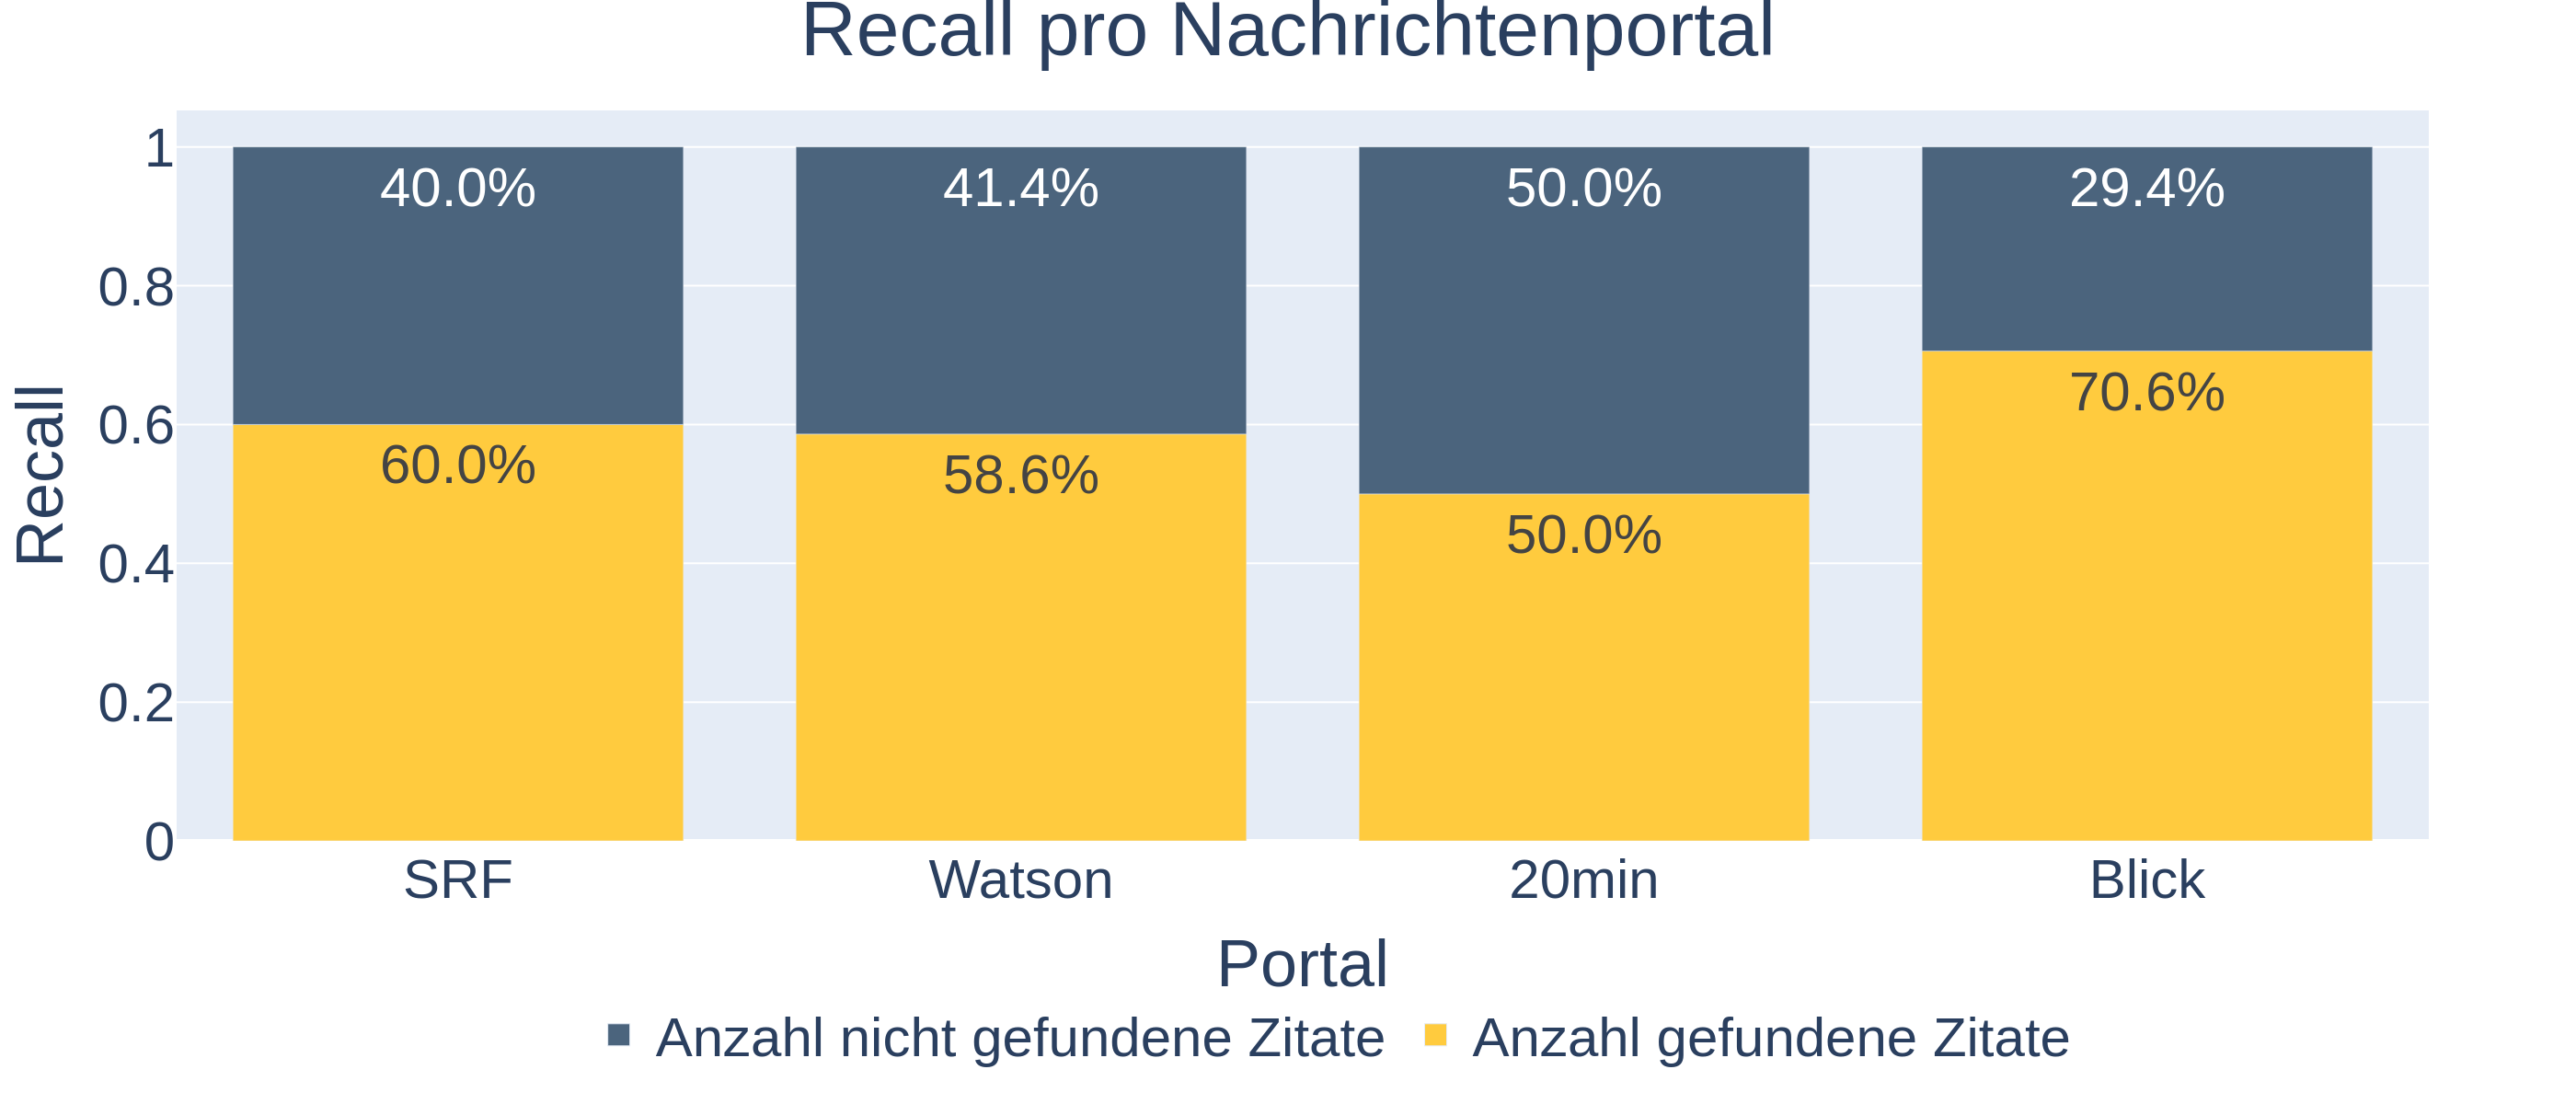
\includegraphics[width=1.0\linewidth]{./images/recall_portals.png}
	\end{center}
	\caption{Recall der Zitate pro Nachrichtenportal}
	\label{barchart-recall}
\end{figure}

\subsection{Qualitätsnote}\label{quality-grade}

Die Qualitätsnote setzt sich aus dem Durchschnitt der Stringähnlichkeiten der extrahierten Zitate
mit der Lösung zusammen. Zum Bestimmen der Stringähnlichkeit verwendet der Algorithmus den
\enquote{SequenceMatcher}\footnote{https://docs.python.org/3/library/difflib.html\#difflib.SequenceMatcher} von Python.
Dieser findet den länsten übereinstimmenden Substring aus zwei Strings relativ zur
Länge der beiden zu vergleichenden Strings.

Die Vermutung, dass die geringe Anzahl Tests Schwankungen in der Qualität verursacht
wird durch den Überblick in den folgenden Diagrammen (vgl. Abbildung \ref{histogram-grades}) gestützt.
20min hat deutlich weniger Zitate in den Lösungen als die anderen Nachrichtenportale.

Die Histogramme legen ausserdem nahe, dass die Rate der False-Positives gering ist.
Denn diese machen sich durch eine tiefe Note bemerkbar, da sie sehr unähnlich zu den Zitaten
aus den Lösungen sind. Dass davon wenige zu erkennen sind, suggeriert, dass False Positives
selten sind.

\begin{figure}[H]
	\begin{tabular}{ll}
		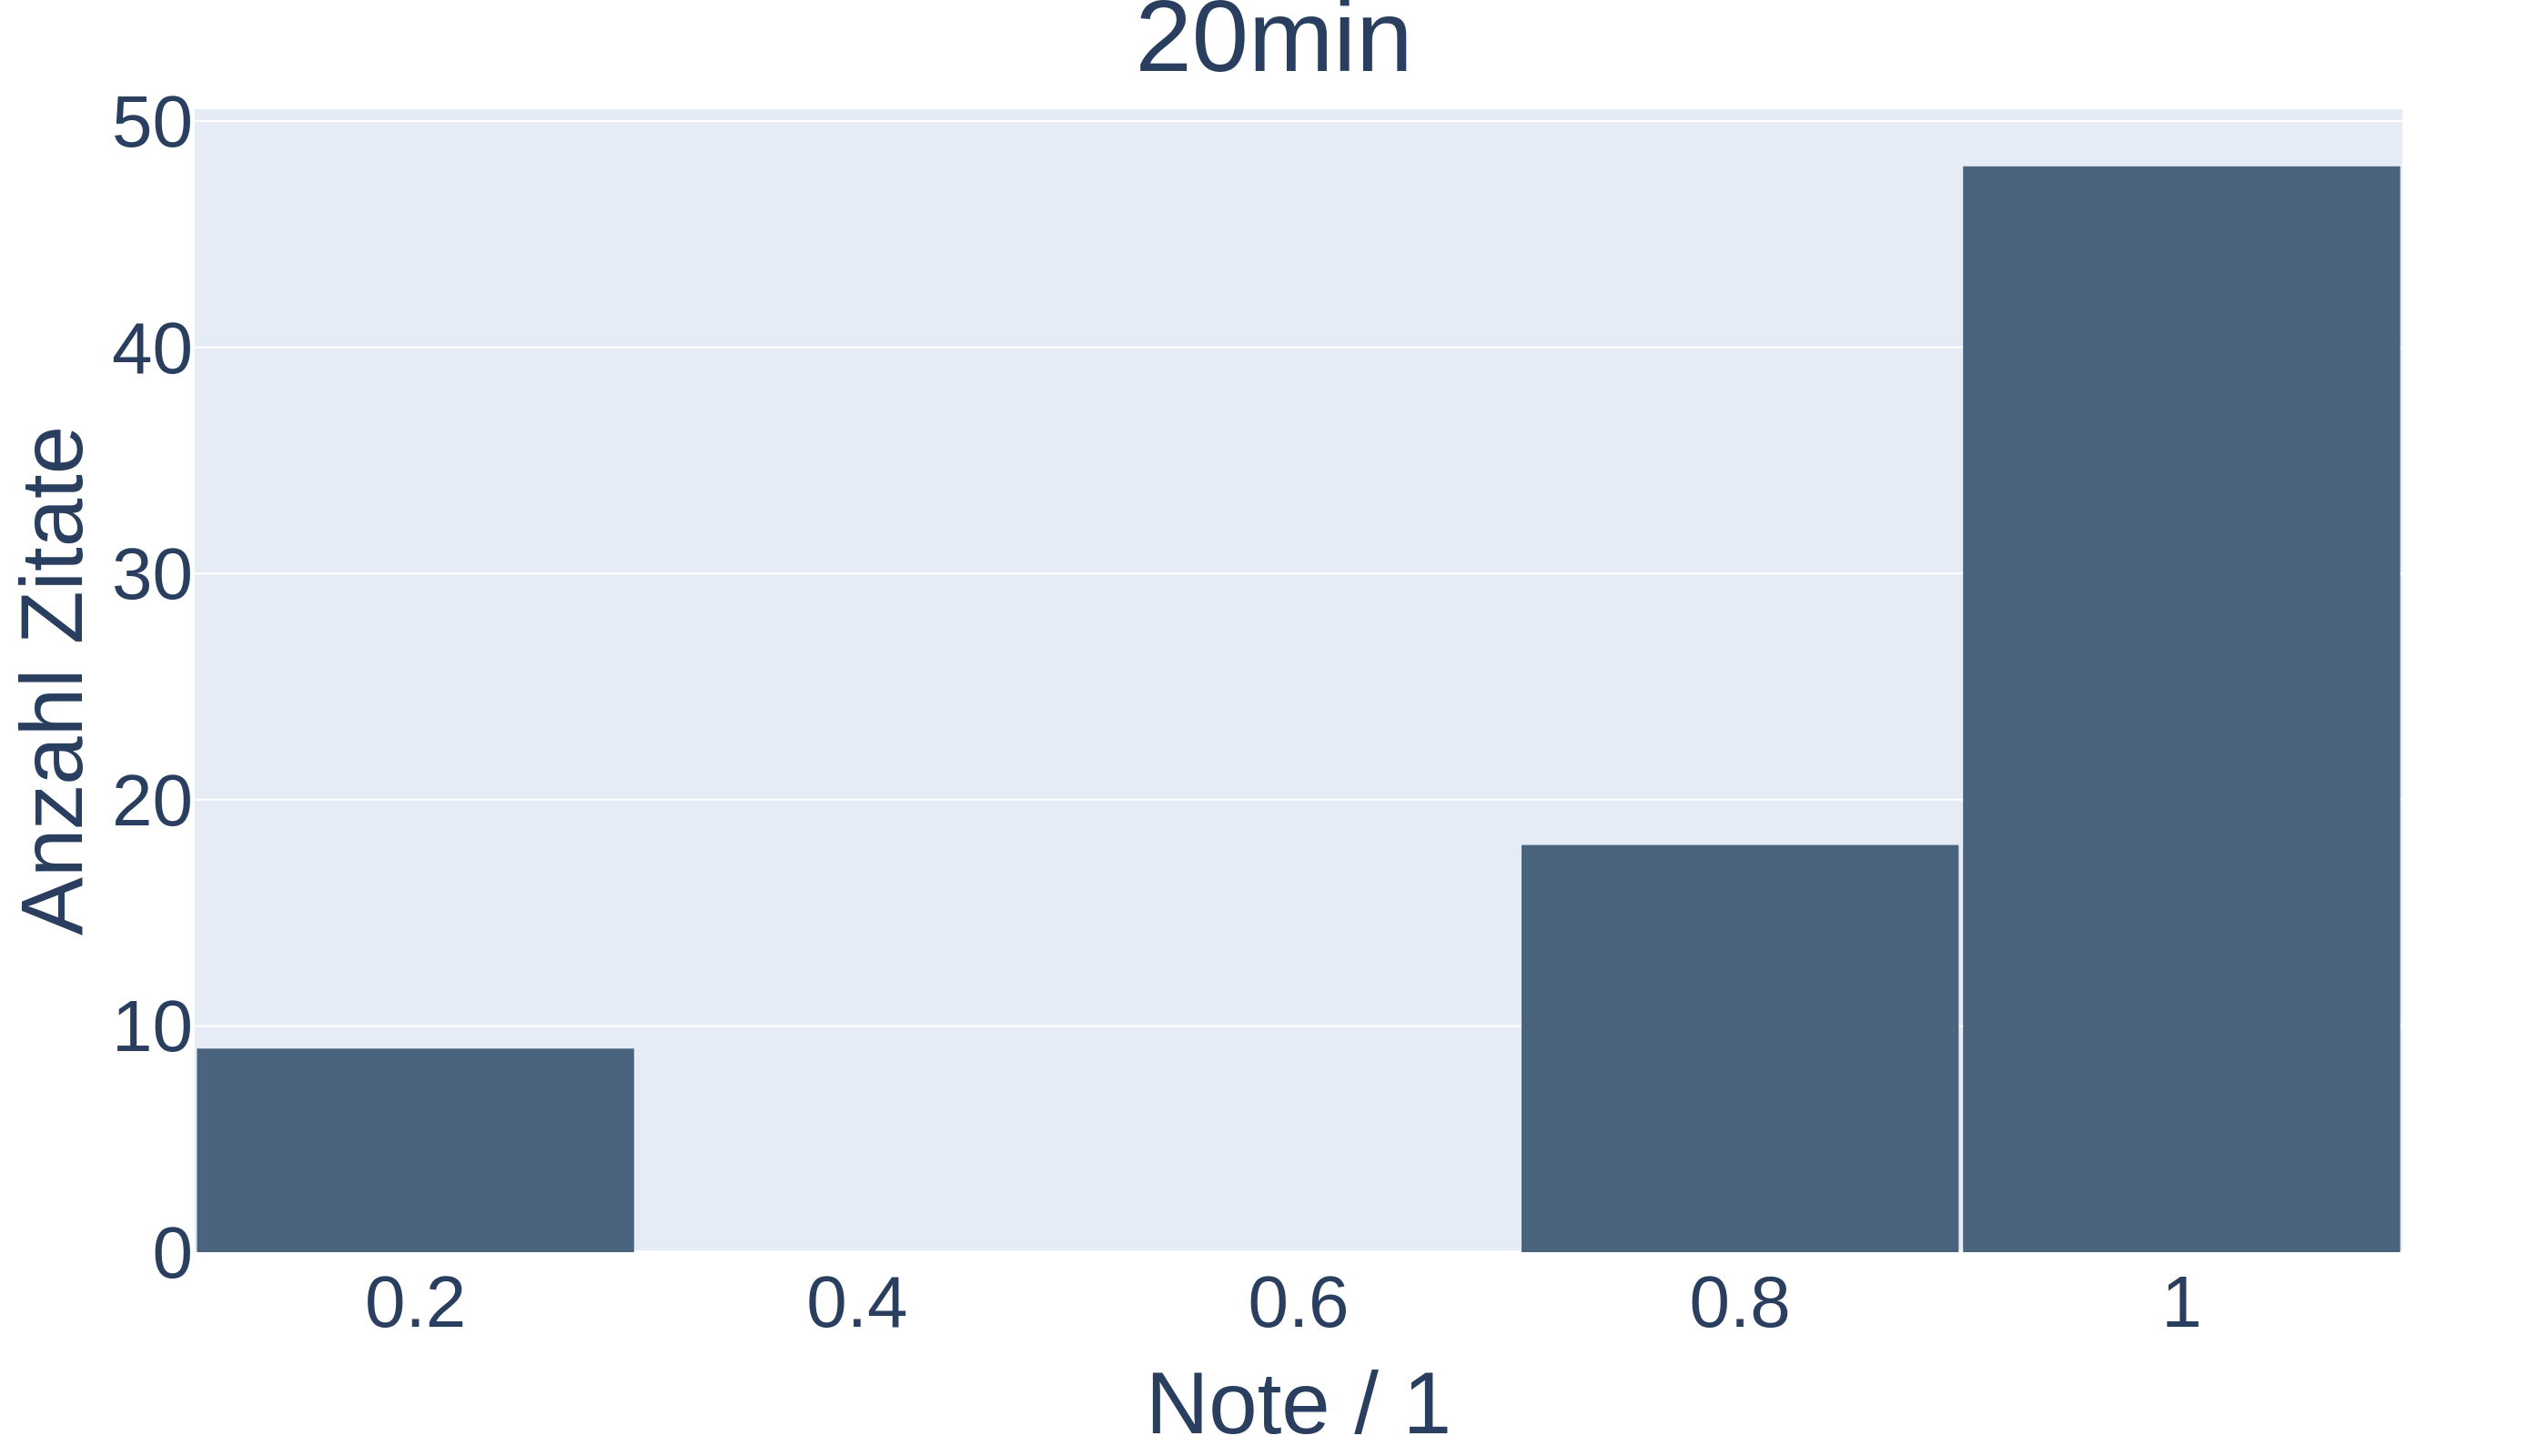
\includegraphics[width=.5\linewidth]{./images/citation_grades_20min.png} & 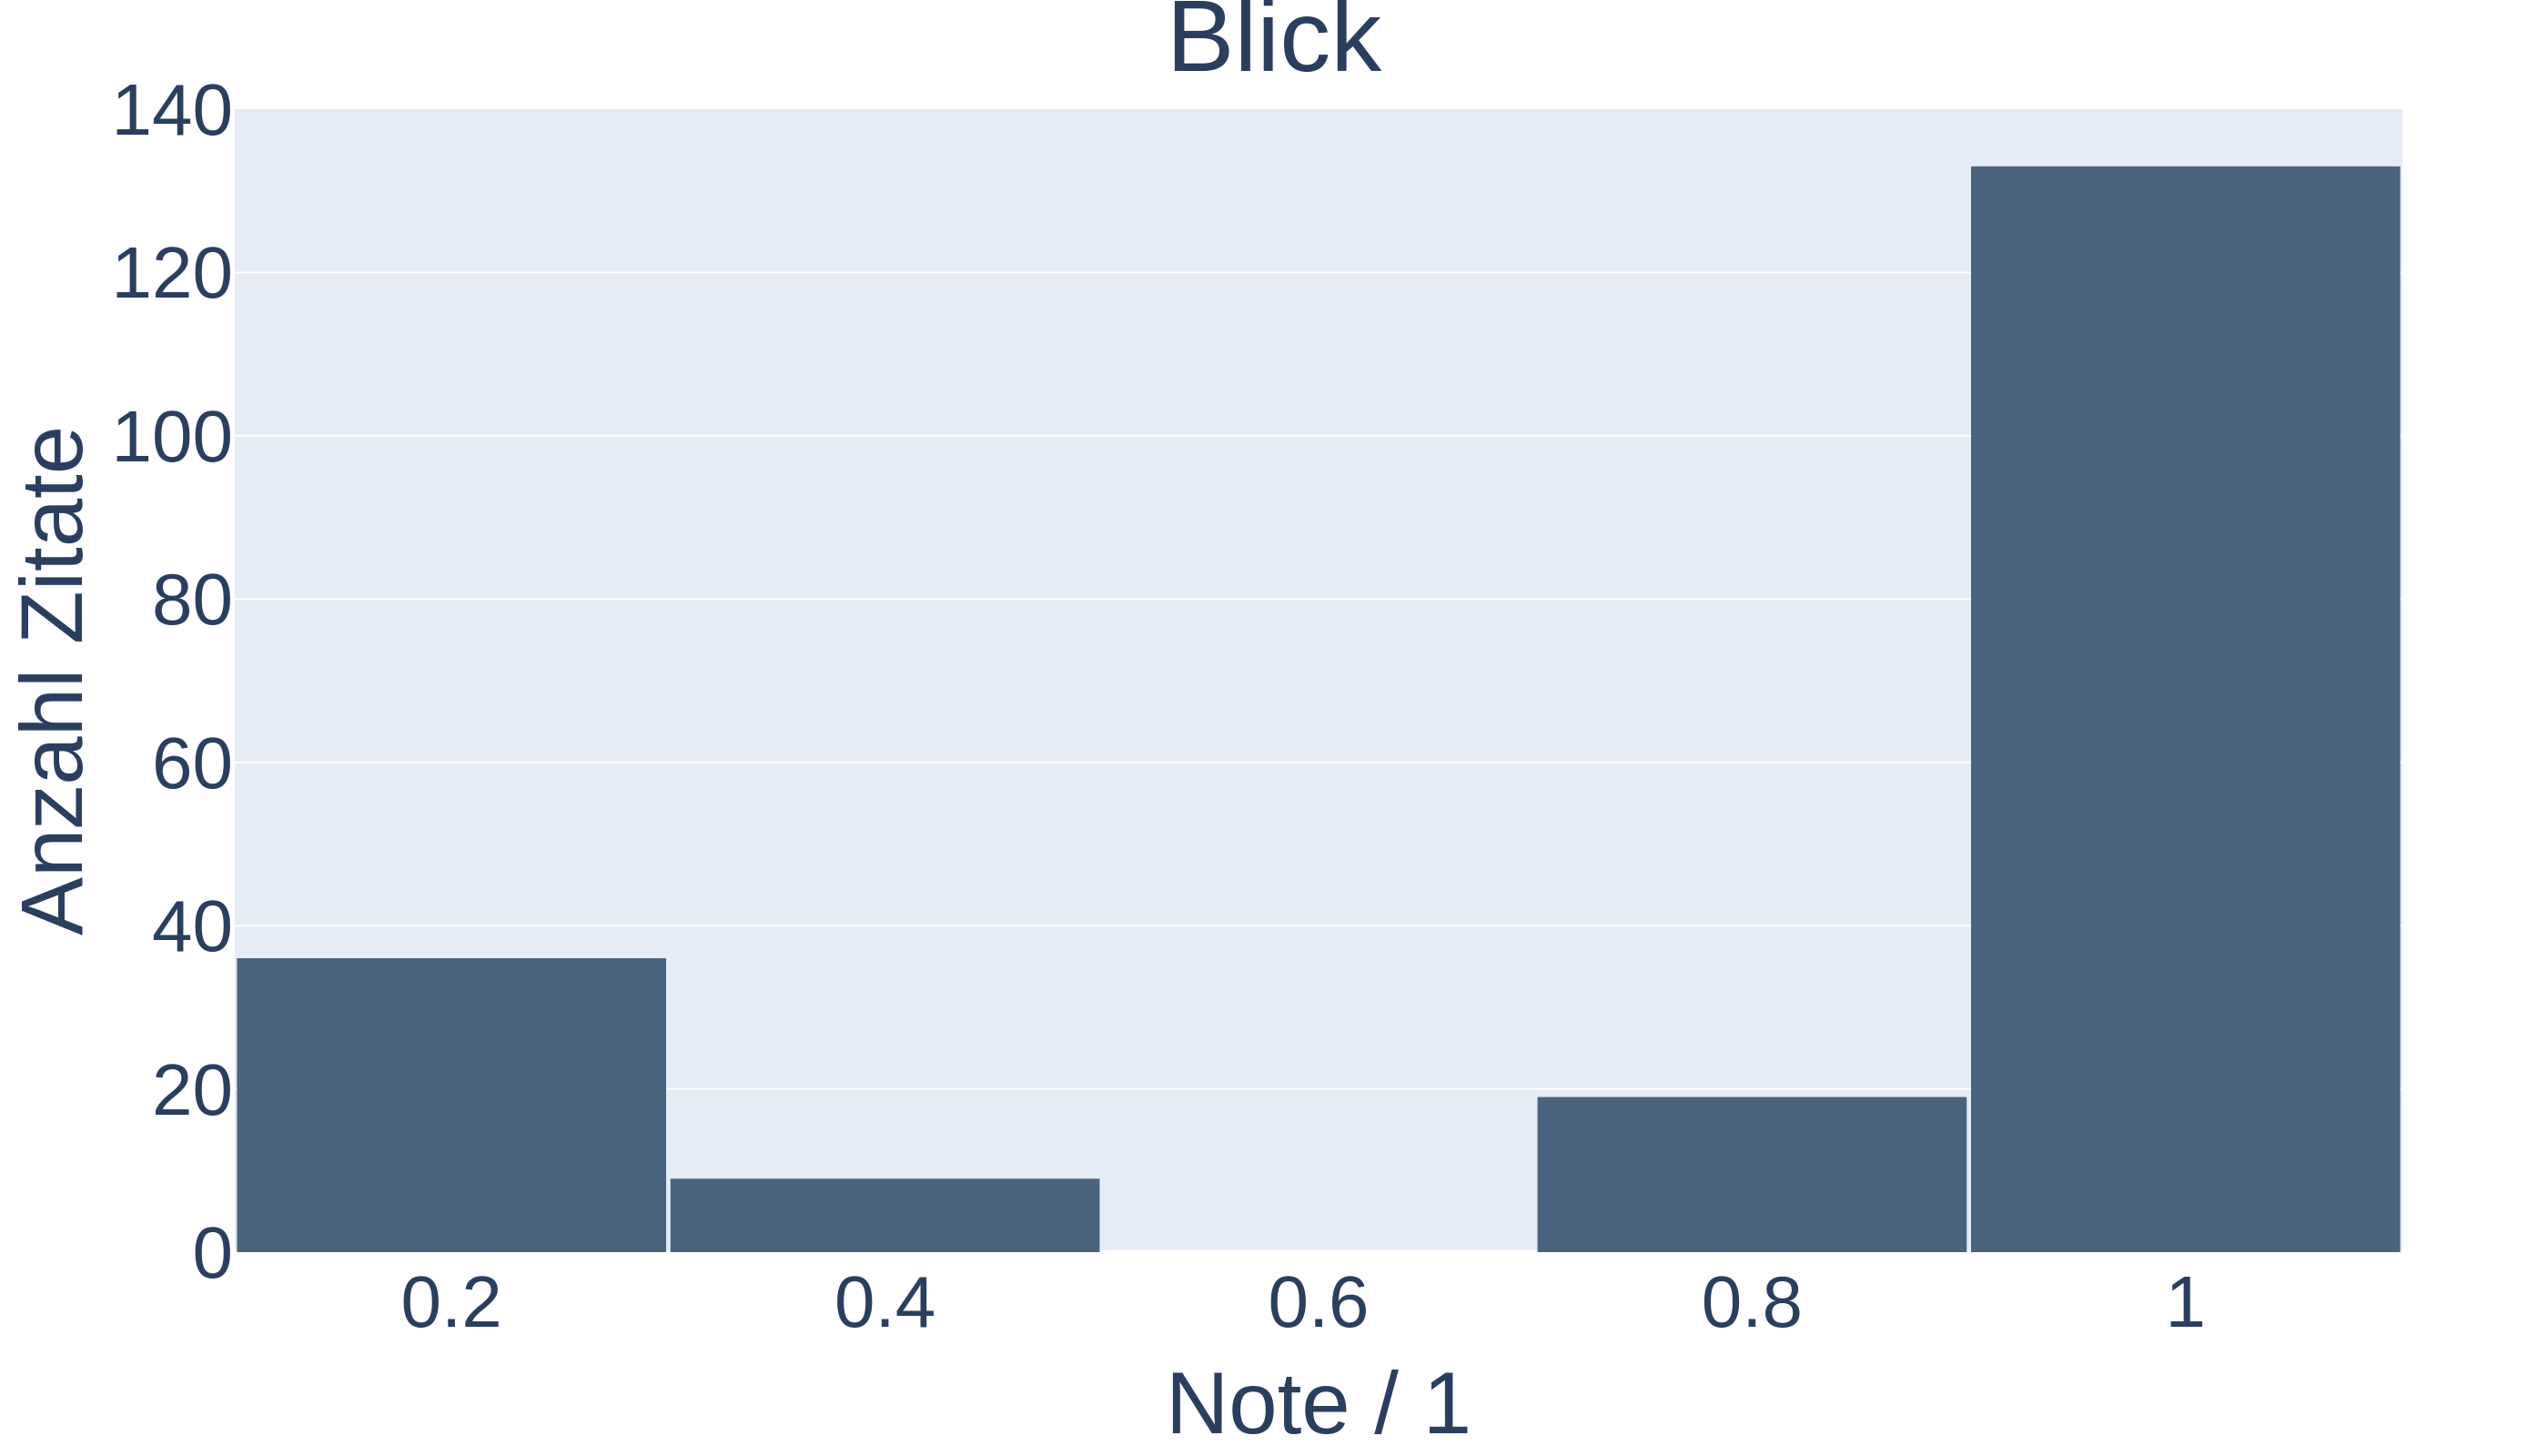
\includegraphics[width=.5\linewidth]{./images/citation_grades_blick.png} \\
		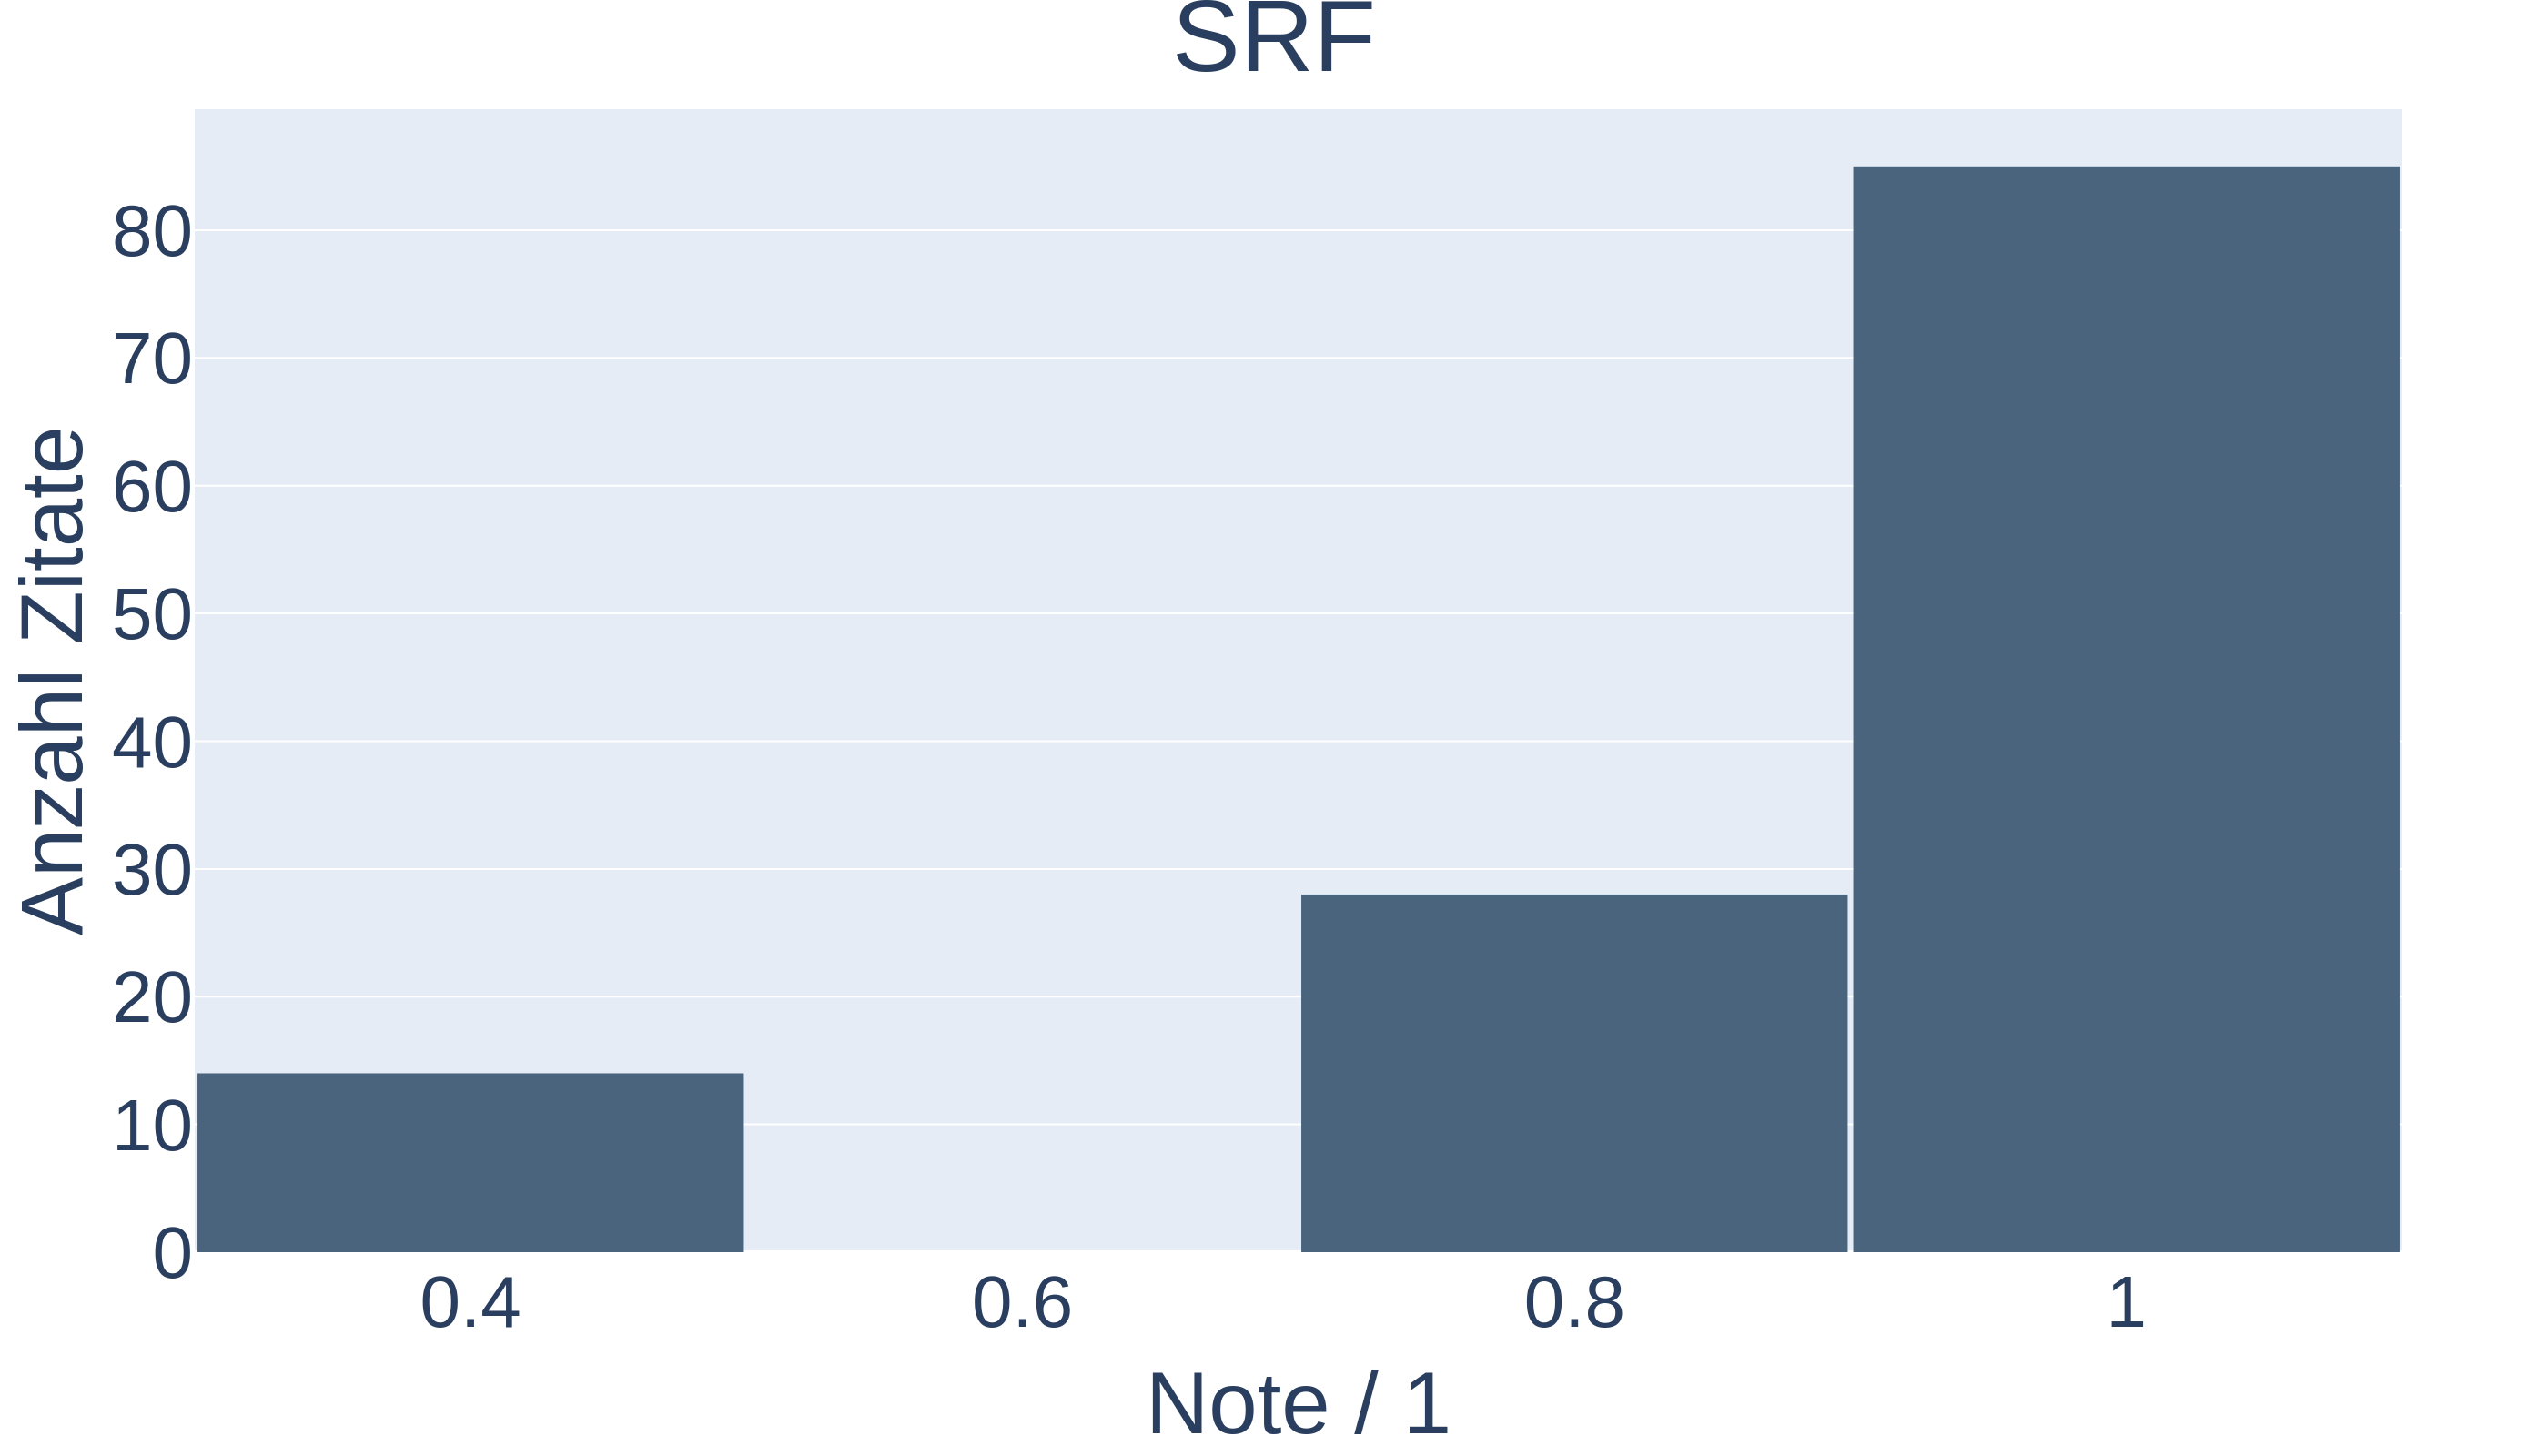
\includegraphics[width=.5\linewidth]{./images/citation_grades_srf.png} & 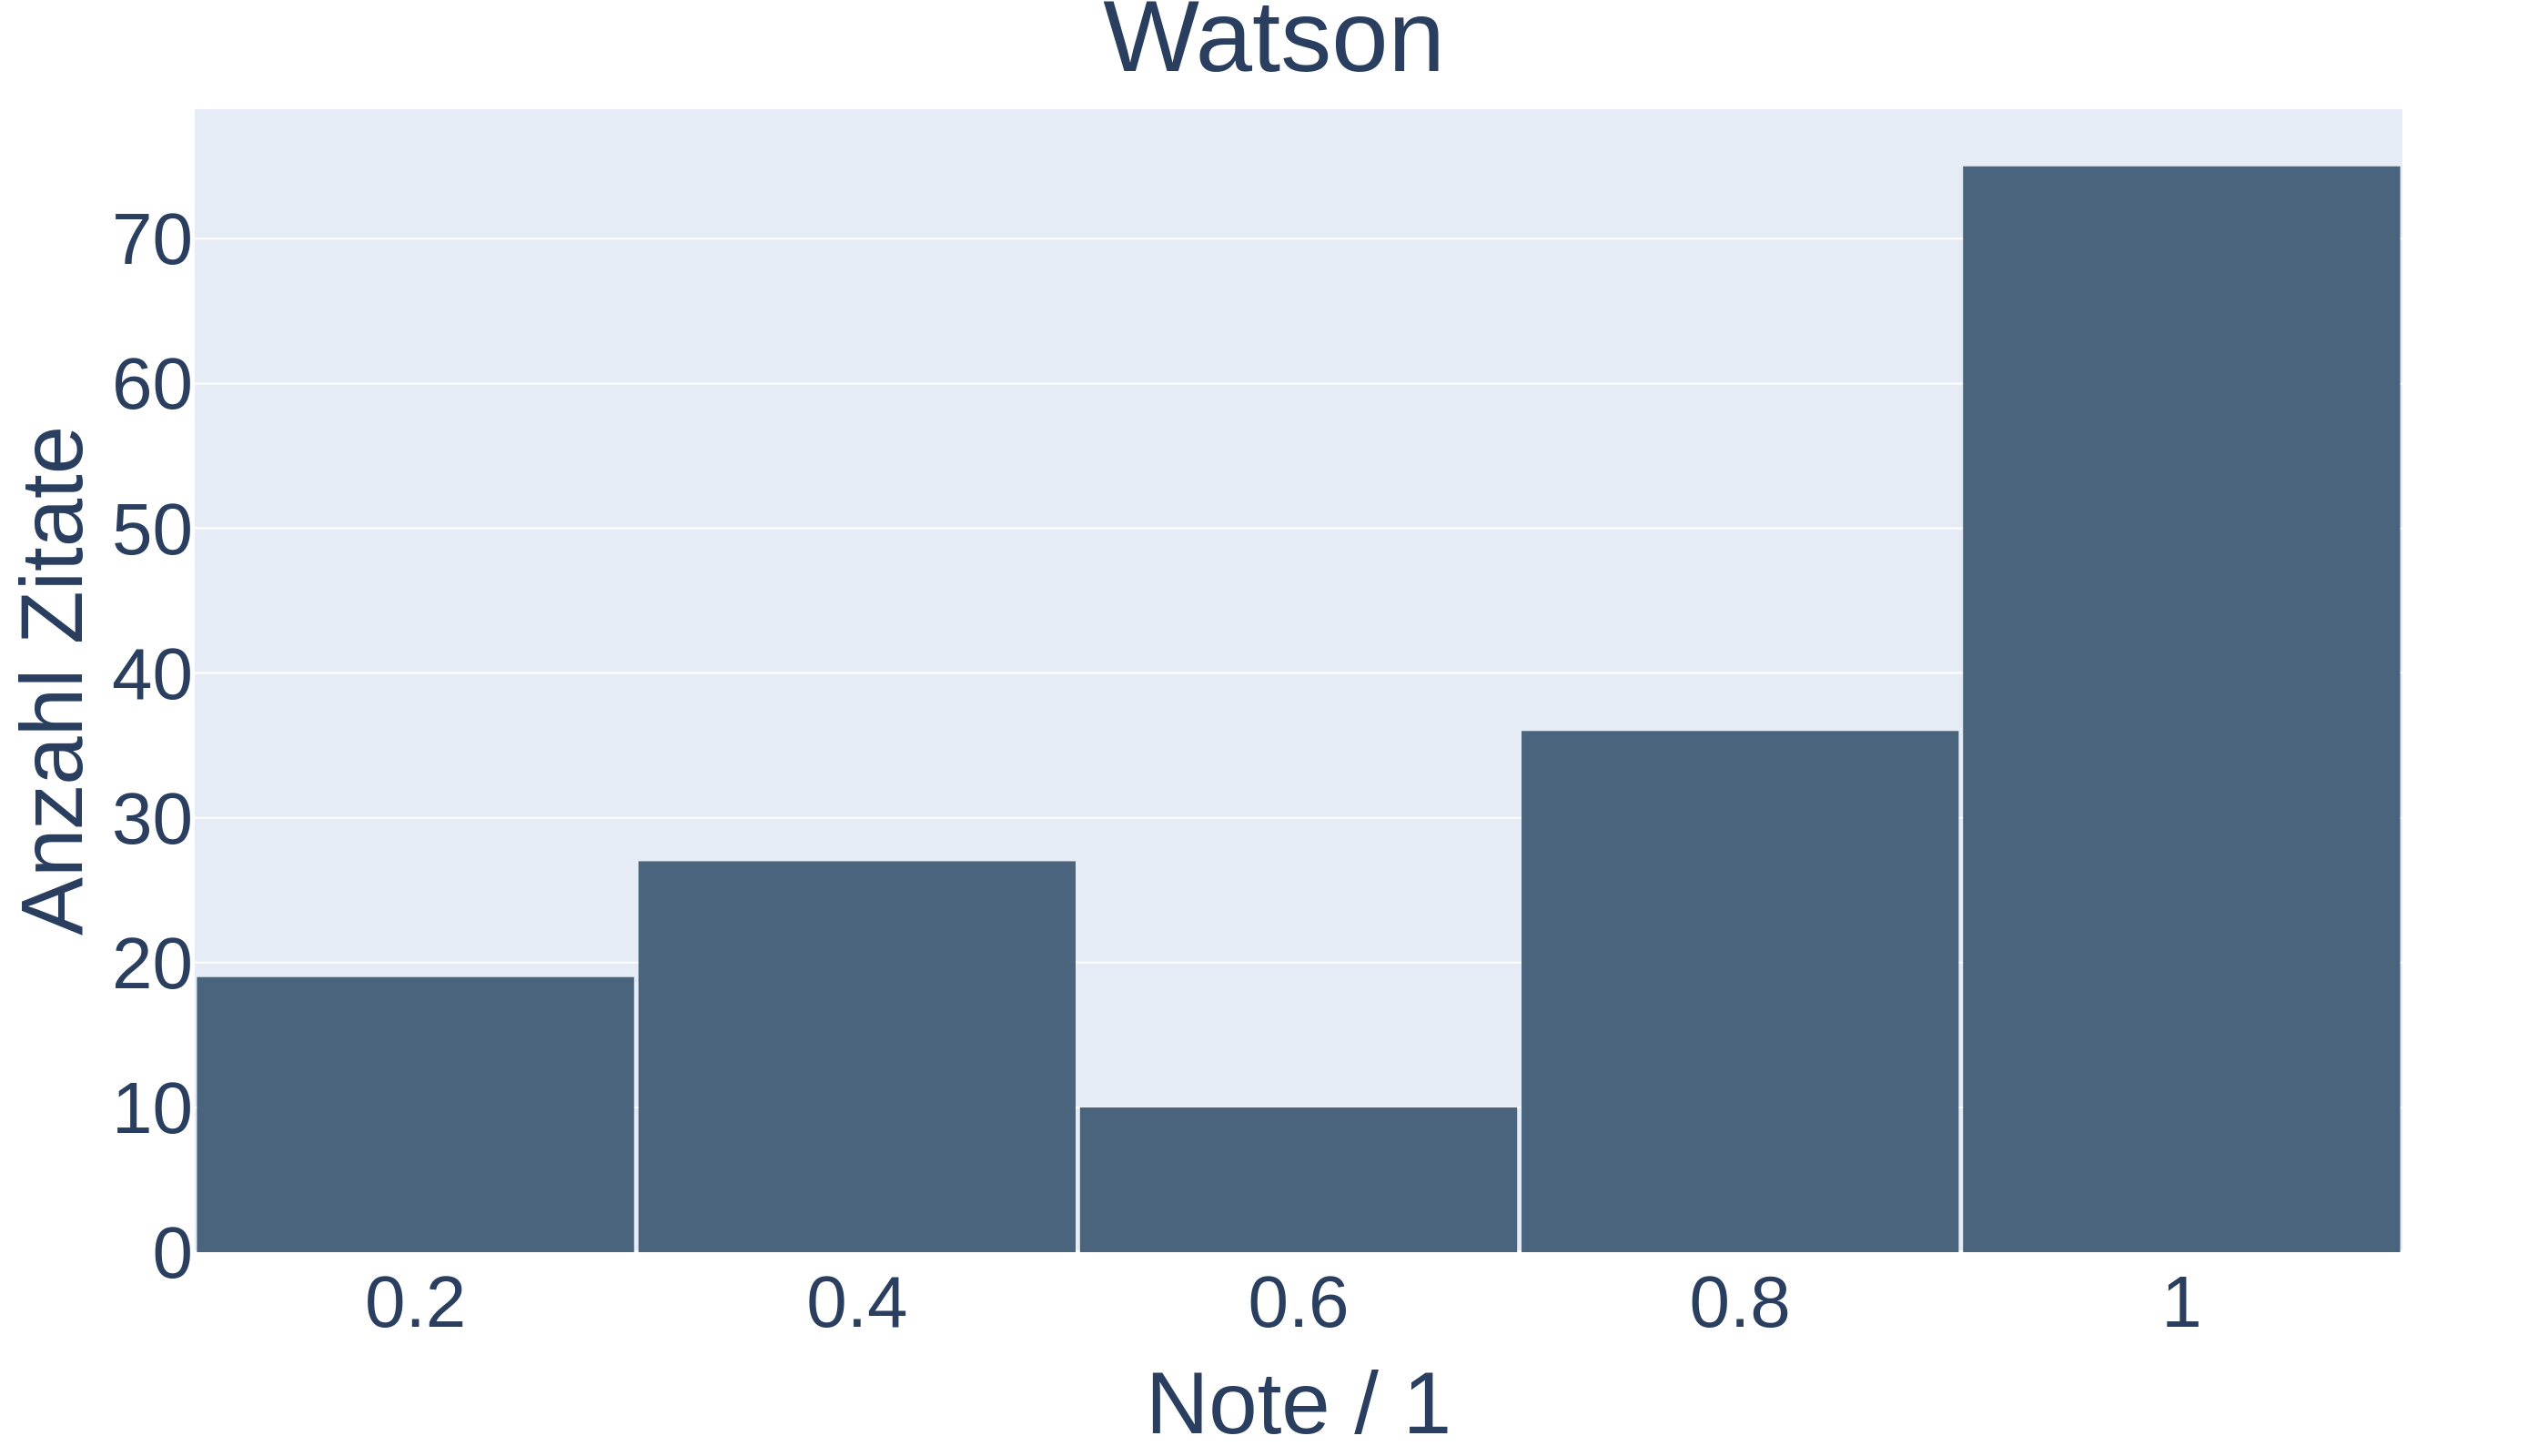
\includegraphics[width=.5\linewidth]{./images/citation_grades_watson.png} \\
	\end{tabular}
	\caption{Histogramme zur Verteilung der Qualität der gefundenen Zitate}
	\label{histogram-grades}
\end{figure}

\subsection{Nicht erkannte Zitate}\label{not-recognized-quotes}

Das nachfolgende Unterkapitel soll einen Überblick über die nicht erkannten Zitate liefern
und erklären, weshalb der Algorithmus aktuell noch nicht in der Lage ist, diese zu erkennen.

Grundsätzlich gibt es viele mögliche Erklärungen, weshalb das Programm gewisse Zitate nicht
erkennen kann. Aufgrund der analysierten Fälle scheinen die meisten fehlenden Zitate
entweder neuen, nicht implementierten Satzstrukturen oder Fehlern des Parsers geschuldet zu sein.

Es hat sich gezeigt, dass der Parser in langen Sätzen mit mehr als zwei Satzteilen
die Abhängigkeiten anders aufbaut. Deshalb wird der Subtree vom Algorithmus ignoriert.
So wird das Zitat einleitende Verb \enquote{schreibt} im folgenden Beispielsatz
als \enquote{mnr} (postnominal modifier) gekenntzeichnet (vgl. Abbildung \ref{citation-with-different-tree-structure-1}).
Wann und wie die gesuchten Verben mit diesem Label auftreten, konnten wir
nicht herausfinden.

\enquote{Dort habe er in einer Wohnung auch einen Grossteil seiner Sachen, unter anderem Familienerbstücke, wie das Inventar aus dem Restaurant Rossberg, wie der «Landbote» schreibt.}

\begin{figure}[H]
	\begin{center}
        \centering
		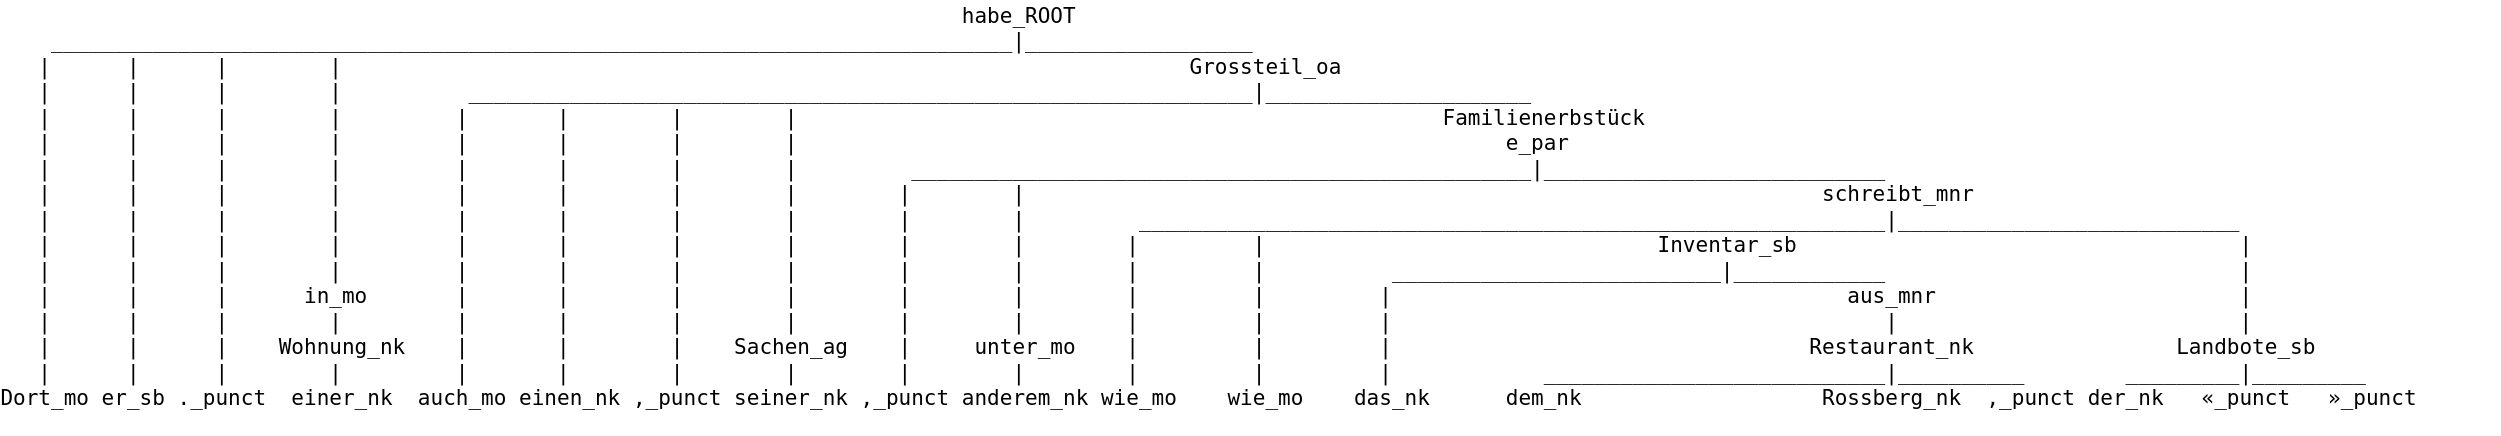
\includegraphics[width=1.0\linewidth]{./images/parse-tree-landbote.png}
	\end{center}
	\caption{Zitat mit anderer Baumstruktur}
	\label{citation-with-different-tree-structure-1}
\end{figure}

Bei dem nachfolgenden Satz wird das signifikante Verb \enquote{mitteilte} als \enquote{mo}
(modifier) gelabelt (vgl. Abbildung \ref{citation-with-different-tree-structure-2}).
In diesem Fall scheint der Parser das Label falsch vergeben zu haben,
denn \enquote{modifier}s werden meist den Adverben und Präpositionen zugeordnet.
Möglicherweise hat der Wortteil \enquote{mit} in diesem Fall den Ausschlag gegeben.

\enquote{Das Departement für Verteidigung, Bevölkerungsschutz und Sport (VBS) wird bis Ende Jahr die rechtlichen Grundlagen erarbeiten, wie der Bundesrat am Mittwoch mitteilte.}

\begin{figure}[H]
	\begin{center}
        \centering
		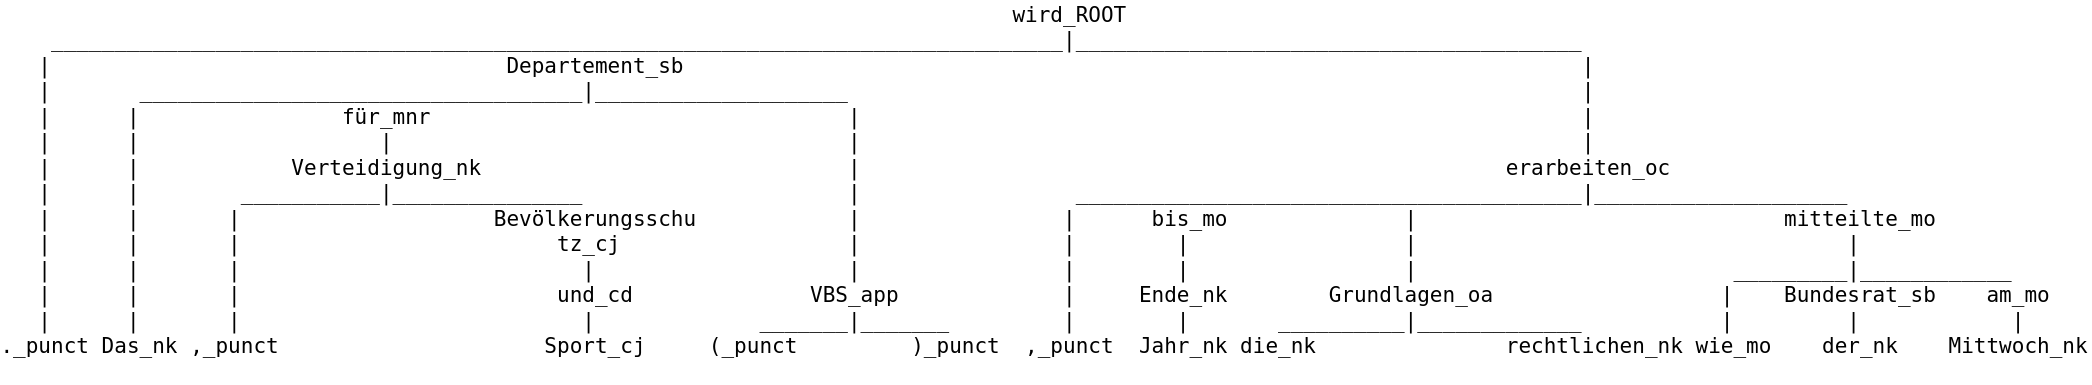
\includegraphics[width=1.0\linewidth]{./images/parse-tree-watson.png}
	\end{center}
	\caption{Zitat mit anderer Baumstruktur}
	\label{citation-with-different-tree-structure-2}
\end{figure}